\documentclass[]{elsarticle}
\usepackage{amsmath}
\usepackage{graphicx}

\usepackage{natbib}
\usepackage[colorlinks,citecolor=red,urlcolor=blue,bookmarks=false,hypertexnames=true]{hyperref} 


\usepackage{tikz}
\usepackage{longtable}
\usepackage{float}
\usepackage{subcaption}
\usepackage{geometry}


\begin{document}

% FRONTMATTER
%%%%%%%%%%%%%%%%%%%%%%%%%%%%%%%%%%%%%%%%%%%%%%%%%%%%%%%%%%%%%%%%%%%%%%%%%%%%%%%%%%%%%%%%%%%%%%%%%%%%%%%%%%%%%%%%%%%%%%%%%%%%%%%%%%%%%

\begin{frontmatter}


\title{Welfare Effects of Individualizing Life-Cycle Investments for Households in Turkey}


\author{Ravshanbek Khodzhimatov\corref{cor1}}
\ead{rsk@ravshansk.com}
\author{Tolga Umut Kuzubaş\corref{cor2}}
\ead{umutkuzubas@gmail.com}
\author{Burak Saltoğlu\corref{cor3}}
\ead{burak.saltoglu@gmail.com}

\cortext[cor2]{Corresponding author}
\address{Boğaziçi University, Department of Economics, Natuk Birkan Building, 34342 Bebek, Istanbul, Turkey}


\begin{abstract}
In this paper, we perform an in-depth welfare comparison of the most common life-cycle investment strategies provided by retirement funds or suggested by classical portfolio theory in the case of households in Turkey. To perform our benchmarking, we constructed heterogeneous agents who worked and invested throughout their lifetime, using parameters calibrated from the historical data. We find that to households with upper-to-middle income, individually customized portfolios result in considerable welfare gains, while ``off-the-shelf'' life-cycle portfolio allocations perform better for households with lower income. We also show that life-cycle investment options outperform ``fixed over the lifetime'' options. 
\end{abstract}


\begin{keyword}
	Life-cycle portfolio decisions, human capital, housing, stock market participation
\end{keyword}


\end{frontmatter}

%INTRODUCTION
%%%%%%%%%%%%%%%%%%%%%%%%%%%%%%%%%%%%%%%%%%%%%%%%%%%%%%%%%%%%%%%%%%%%%%%%%%%%%%%%%%%%%%%%%%%%%%%%%%%%%%%%%%%%%%%%%%%%%%%%%%%%%%%%%%%%%

\section{Introduction} % Main chapter title
\label{intro} % For referencing the chapter elsewhere, use \ref{introduction} 

The field of financial economics has gone through big changes since its foundation by \citet{markowitz} and \citet{tobin}. They pioneered the mean-variance analysis, which, given some assumptions, suggested that if investors cared about maximizing returns (mean) and minimizing risks (variance), then the optimal ratio of stocks to bonds in a single-period portfolio would be fixed for everyone, the share of former being equal to:

\begin{equation}
	\alpha = \frac{E[R] - R_f}{\gamma\sigma^2}
\end{equation}

\citet{merton} generalized the problem to multiple periods using dynamic programming and found that it is optimal for all households to repeat the same fixed mean-variance solution every period.

These results were inconsistent with the popular financial advice suggesting that younger investors should have higher share of stocks in portfolio, and older investors --- higher share of bonds. This advice was summarized by the famous rule of thumb:

\begin{equation}
	\alpha_t = (100 - t)\%
\end{equation}

Although \citet{samuelson} denied that risk-aversion changes by age, dismissing this advice would question the rationality of investors and ``constitute \textit{prima facie} evidence that people do not optimize'' (\citet{canner}).

\citet{bodie} solved this problem by adding human capital into the \citet{merton}'s dynamic model and found that for complete markets and constant risk-free labor income, the optimal share of stocks in a portfolio is:

\begin{equation}
	\alpha_t = \frac{\mu - R_f}{\gamma \sigma^2}(\frac{W_t + H_t}{W_t})
\end{equation}

Steady depletion of human capital through life explained the higher share of stocks in younger people. \citet{cgm} extended this idea to the case of variable labor income, to find a recursive solution which could be approximated by the following rule of thumb:

\begin{equation}
	\alpha_t =
	\begin{cases}
		100\% 			& 	t<40\\
		(200-2.5t)\% 	& 	t\in[40,60]\\
		50\% 			& 	t>60
	\end{cases}
\end{equation}


However, the hump-shaped lifetime stock share graph, observed by \citet{chang} of Richmond Fed (see Figure \ref{fig:chang}) instead of expected downward sloping one, suggested the presence of an opposing force.

\begin{figure}[h!]
	\centering
	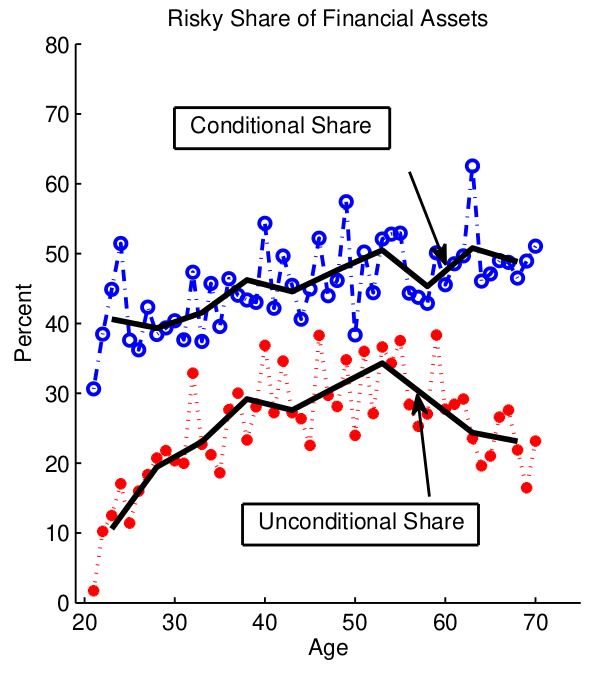
\includegraphics[scale=0.3]{figs/scf.png}
	\caption{Hump-shaped unconditional lifetime stock share. Source: \citet{chang}}
	\label{fig:chang}
\end{figure}

\citet{cocco} found that this force was housing investment, which, due to its large size, crowded out all stocks from younger investors' portfolios. \citet{flavin} supported this view by showing that younger people, who already own the house, tend to invest more aggressively, as expected by \citet{bodie}.

\citet{munk} found the same patterns using a series of one-period mean-variance optimizations without any dynamic stochastic modeling tools. He stated that in presence of housing, the optimal stock ($\pi$) and housing ($\pi_h$) shares can be solved analytically as follows:

\begin{subequations}
	
	\begin{equation}
		\pi_{t+1} = \frac{1}{\gamma (1 - \rho^2_{SH}) \sigma_S} \cdot \frac{W_t}{F_t} \left( \frac{\mu_s - r_f}{\sigma_S} - \rho_{SH} \frac{\mu_h - r_f}{\sigma_h} \right) - \frac{L_t}{F_t} \cdot \frac{\sigma_L}{\sigma_S} \frac{\rho_{SL} - \rho_{SH}\rho_{HL}}{1 - \rho^2_{SH}}
	\end{equation}

	\begin{equation}
		\pi_{h,t+1} = \frac{1}{\gamma (1 - \rho^2_{SH}) \sigma_H} \cdot \frac{W_t}{F_t} \left( \frac{\mu_h - r_f}{\sigma_h} - \rho_{SH} \frac{\mu_s - r_f}{\sigma_s} \right) - \frac{L_t}{F_t} \cdot \frac{\sigma_L}{\sigma_h} \frac{\rho_{HL} - \rho_{SH}\rho_{SL}}{1 - \rho^2_{SH}}
	\end{equation}

\end{subequations}
	
Finally, \citet{ascheberg} illustrated the existence of long-term cointegration among house prices, stock prices, and labor income, the fact often omitted by previous portfolio researches for simplicity. Therefore, in our analysis we will not neglect the correlations as being equal to zero. 

In this paper, we calculate the wealth accumulated from lifetime investments given by all the strategies above and suggested by current Turkish banks. We benchmark the resulting welfare for heterogeneous agents in Turkey with varying sectors, levels of education and risk-aversion. We conclude with the separate investment advice for all types of households mentioned above.

The remainder of the paper is organized as follows: Section \ref{model} presents the theoretical framework we will use in our analysis. Section \ref{data} contains detailed information about our data sources, parameter calibration and solves for the optimal investment strategies. Section \ref{welfare} does the welfare benchmarking of every investment option for every agent, and Section \ref{conclusion} concludes.

% THEORETICAL FRAMEWORK 
%%%%%%%%%%%%%%%%%%%%%%%%%%%%%%%%%%%%%%%%%%%%%%%%%%%%%%%%%%%%%%%%%%%%%%%%%%%%%%%%%%%%%%%%%%%%%%%%%%%%%%%%%%%%%%%%%%%%%%%%%%%%%%%%%%%%%

\section{Theoretical framework}
\label{model}

\subsection{House prices, stock prices and labor income series}
In accordance with \citet{ccgm} and \citet{olear} we model the labor income process as a function of individiual characteristics $f(t, Z_{it})$ plus idiosyncratic shocks $v_{it}$. Upon reaching the retirement age $T$, an individual receives a certain percentage $\lambda$ of his/her last wage:

\begin{equation}
	Y_{i,t+1} = 
	\begin{cases}
		Y_{it} (1 + \Delta f(t+1,Z_{i,t+1}) + v_{it}), 	& t \leq T \\
		\lambda (1 + f(T, Z_{iT}) + v_{iT}), 			& t > T
	\end{cases}	
\end{equation}

We model house prices and stock prices as time series satisfying the discrete version of \citet{ascheberg}'s stock, housing and labor income correlation structure, mentioned in \ref{ascheberg}:


\subsection{Calibration}

We calibrate the above parameters using data obtained from the repeated cross-sectional study by \citet{tuik}. In line with \citet{aktug} we aggregate these studies to obtain a pseudo-panel, which we will use to summarize labor income dynamics.

In summarizing the series we will use simple medians and means. In determining the expected values of time-series parameters, we will use simple arithmetic mean and standard deviation.

\paragraph{}
In constructing the simulated labor income series, we used kinked ordinary least-squares (OLS) estimations with kinks at ages of 35 and 45 separately for every education level $i$:

\begin{center}
	$\Delta\log (wage_{it}) = \alpha_0 + \alpha_1 \cdot d_{35} + \alpha_2 \cdot d_{45} + \alpha_3 \cdot t$
\end{center}




\subsection{Welfare measurement}
Similarly to Cocco et al. (2005) we use CRRA utility function in our model:

\begin{center}
	$E_1[U(c)] = E_1 \left[\displaystyle\sum^T_{t=1} \delta^{t-1} \displaystyle\prod^{t-1}_{j=0} p_j \cdot \frac{c^{1-\gamma}_{it}}{1-\gamma}\right]$
\end{center}

where $p_k$ is the probability of survival from time $k-1$ to time $k$. Note that we omitted the bequest motives from the original formulation, thus retired person consumes all of his income at any given time.

%\paragraph*{}Following Olear (2016) we use certainty equivalent consumptions (CEC) instead of expected utilities to compare the welfare effects between different lifecycle choices. Appendix C shows the calculation of the following formula for CEC:

%\begin{center}
%	$CEC = \left( \frac{E[U(c)]\cdot(1-\gamma)}{\sum^T_{t=1} \delta^{t-1} \prod^{t-1}_{j=0} p_j} \right)^{1/(1-\gamma)}$
%\end{center}


\subsection{Individualization}

To derive the individual lifecycle portfolios for every wealth type we use a special case of Munk (2016) with housing investment and human capital included. The similar approach and its solution has been done by Olear (2016), but she included housing capital as a pre-existing wealth bought for an outside mortgage, independent of the investment decision. In this paper, we consider housing as a purely financial investment, in line with Munk (2016). Munk provides the following optimal asset allocation:


\begin{center}
	$\pi_{t+1} = \frac{\mu_s - r_f}{\gamma \sigma^2_s}  + \frac{L_t}{F_t} \cdot \left(\frac{\mu_s - r_f}{\gamma \sigma^2_s} - \frac{\rho_{SL}\sigma_L}{\sigma_S} \right)$
\end{center}

without housing investment, and:

\begin{center}
	$\pi_{t+1} = \frac{1}{\gamma (1 - \rho^2_{SH}) \sigma_S} \cdot \frac{W_t}{F_t} \left( \frac{\mu_s - r_f}{\sigma_S} - \rho_{SH} \frac{\mu_h - r_f}{\sigma_h} \right) - \frac{L_t}{F_t} \cdot \frac{\sigma_L}{\sigma_S} \frac{\rho_{SL} - \rho_{SH}\rho_{HL}}{1 - \rho^2_{SH}}$\\
	$\pi_{h,t+1} = \frac{1}{\gamma (1 - \rho^2_{SH}) \sigma_H} \cdot \frac{W_t}{F_t} \left( \frac{\mu_h - r_f}{\sigma_h} - \rho_{SH} \frac{\mu_s - r_f}{\sigma_s} \right) - \frac{L_t}{F_t} \cdot \frac{\sigma_L}{\sigma_h} \frac{\rho_{HL} - \rho_{SH}\rho_{SL}}{1 - \rho^2_{SH}}$
\end{center}

when housing is considered as a second risky financial investment. In line with Munk (2016), we calculate the risk free asset share as $\left( 1 - \pi - \pi_h \right)$ and only then impose constraints. If any of the above shares is negative, we equate it to zero, and if the sum of remaining shares exceeds $1$, we divde all of the shares by their sum to obtain a proportionate asset allocation. 

\subsection{Retirement income}

The funds invested in retirement are modeled to be paid back in annuities. Thus, we ignore the case when some share of matured fund can be withdrawn immediately. Further, in order for our individualization analysis (based on house posessions) to have an effect, we also use reverse mortgages proposed. In theory, reverse mortgages pay retired individuals fixed annuity in return for inheriting the house after she dies. This is a plausible tool, because we ignore all bequest motives, and it liquidifies the housing posessions, although it is not yet available for Turkish investors. 

\paragraph{}So, at the age of 57, the price of owned house is calculated and is added to the matured pension amount ($MP$) to obtain total wealth:

\begin{center}
	$W_{57} = H_{57} + MP$
\end{center}

All of the $W_{57}$ is used to buy an annuity which will repay an individual $\frac{W_{57}}{1+\sum^{100}_{t=58} \frac{p_t}{1+r_f}}$ annually. The calculation details are available in Appendix D. 

% DATA AND SIMULATION
%%%%%%%%%%%%%%%%%%%%%%%%%%%%%%%%%%%%%%%%%%%%%%%%%%%%%%%%%%%%%%%%%%%%%%%%%%%%%%%%%%%%%%%%%%%%%%%%%%%%%%%%%%%%%%%%%%%%%%%%%%%%%%%%%%%%%
\section{Data and simulation}
\label{data}

In our simulation we will compare welfare effects of default lifecycles and individualized lifecycles defined below. The magnitutes and sources of parameters are given in the next section. Default lifecycles are taken from the ones mentioned in our Literature Review chapter and from the real investment strategies of the largest Turkish pension fund provider Anadolu Hayat Emeklilik. Individualized lifecycles will be calculated using Munk's optimal portfolio formula from previous chapter taking idiosyncracies into consideration.

\subsection{Data}

To measure the stock series we used BIST 30 index which measures the aggregate performance of 30 best companies in Turkey. The monthly data is taken from Borsa Istanbul. We can see from Figure 4.1 the general upward trend with collapse during 2008 crisis.

\begin{figure}
	\centering
    \begin{minipage}{0.45\textwidth}
		\centering
		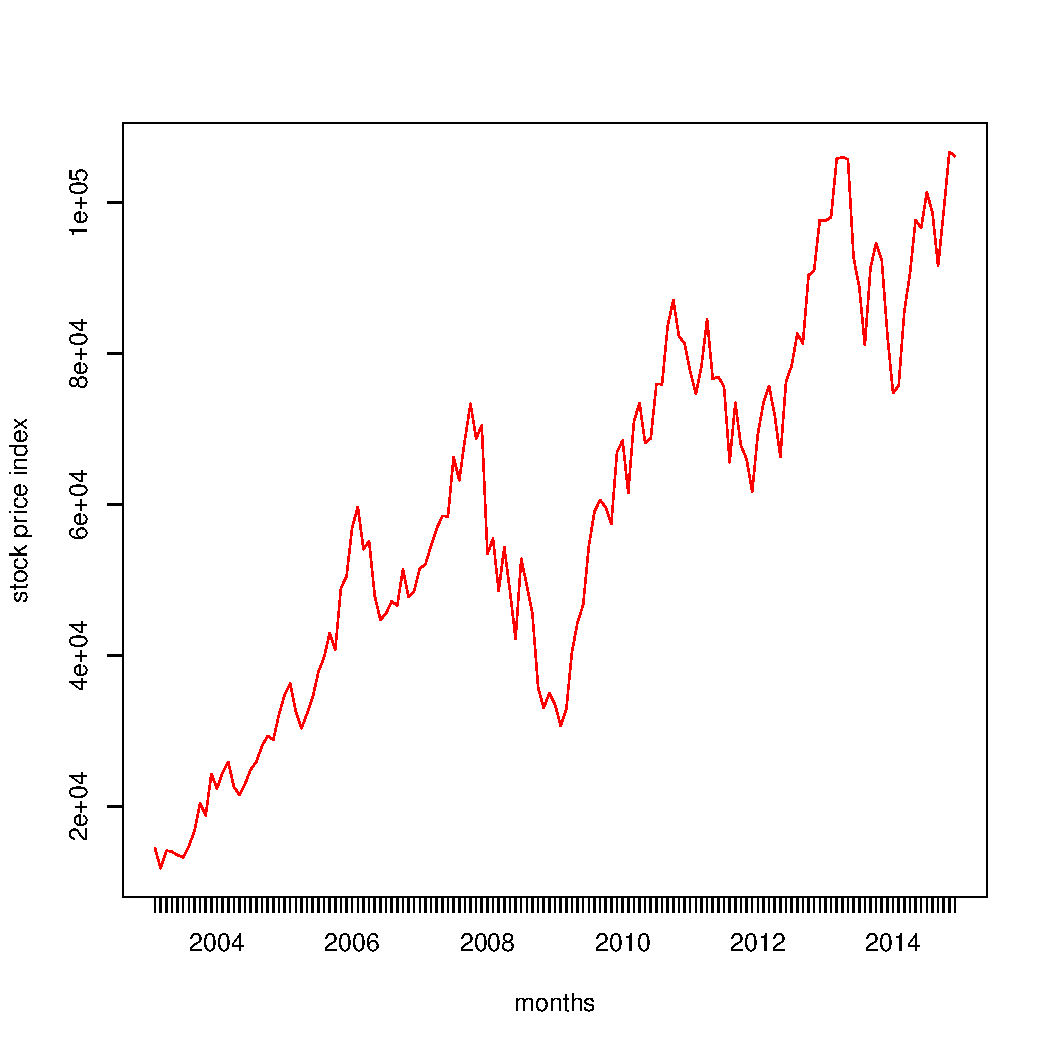
\includegraphics[scale=0.4]{figs/bist.pdf}
		\caption{BIST30 Turkish stock market performance index}
	\end{minipage}
	\hfill
    \begin{minipage}{0.45\textwidth}
		\centering
		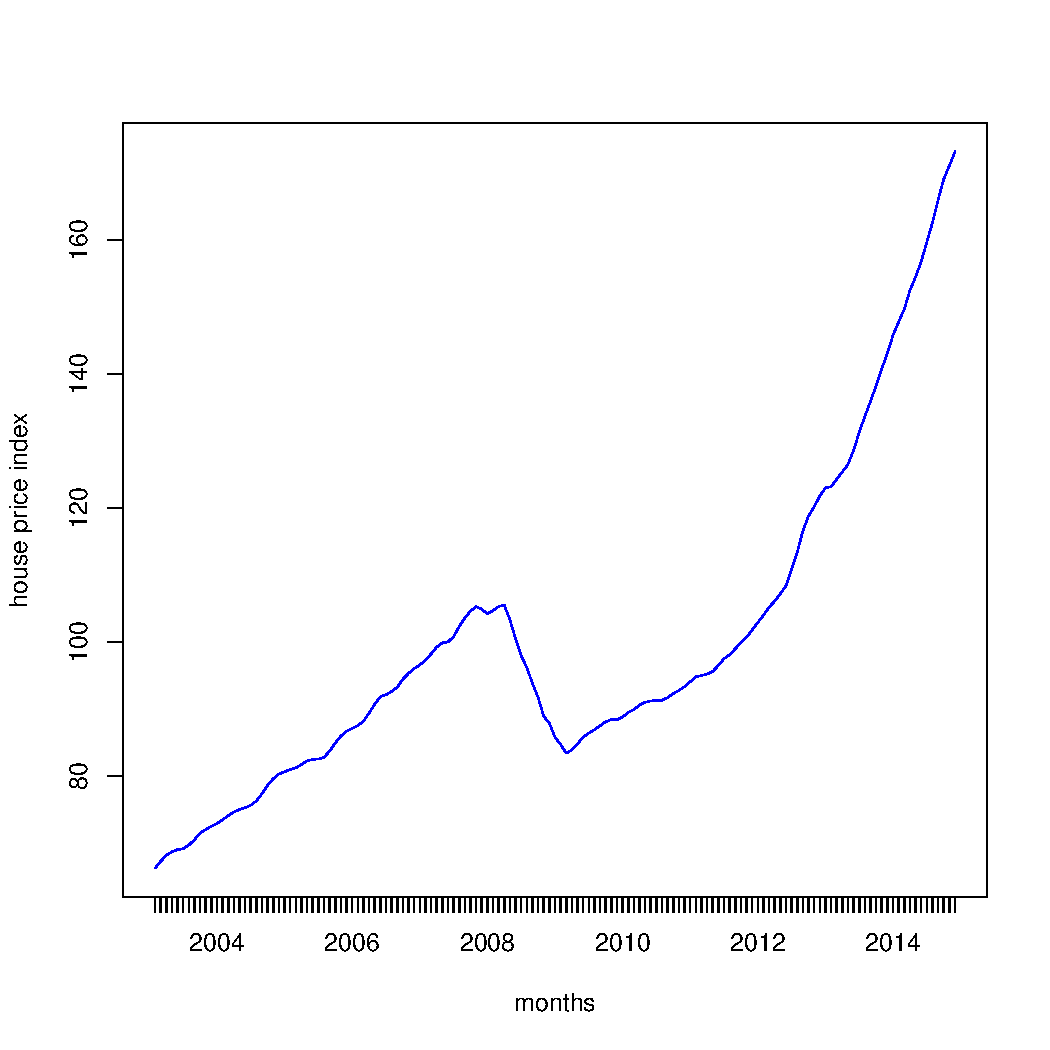
\includegraphics[scale=0.4]{figs/reidin.pdf}
		\caption{Reidin Turkish house price index}
	\end{minipage}
\end{figure}

\paragraph{}We used Reidin AEINDEXF index to obtain data on house prices in Istanbul. The historical dynamics of this index are illustrated in Figure 4.2.

\paragraph{}We used TUIK's Household Budget Survey Data and regression results of Aktug, Kuzubas, Torul (2017). We have 55 thousand panel data points for 170 households for 2001 to 2014 years. We can observe the hump-shaped lifetime income distribution in Figure 4.3. This corresponds well to an established literature in this field.

\begin{figure}[h]
	\centering
	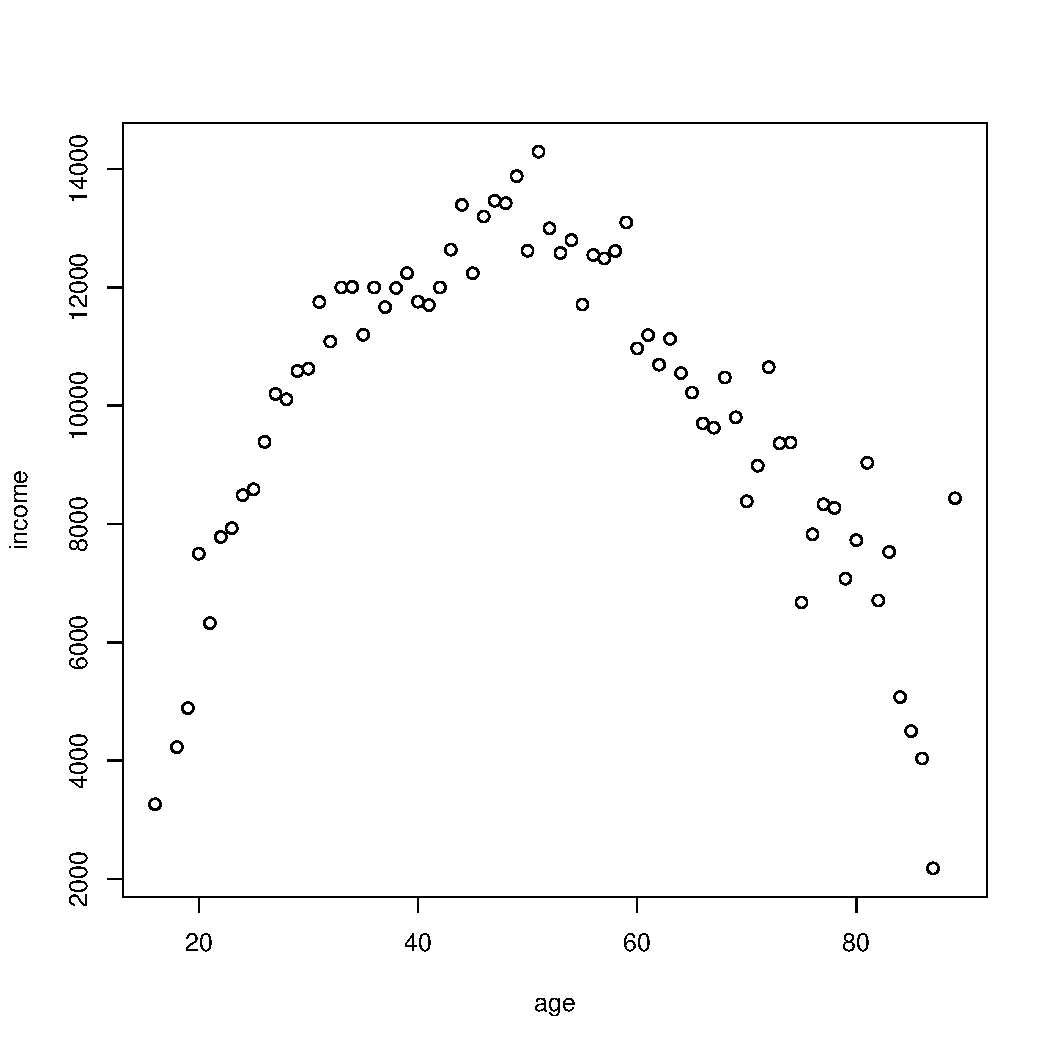
\includegraphics[scale=0.6]{figs/wage2median.pdf}
	\caption{Median Turkish salaries by age}
\end{figure}

\subsubsection{Default parameters}
In our simulation we start with a 28 years old individual who invests in her retirement for 30 years until she reaches retirement at 57. We set the default coefficient of relative risk aversion at $5$, but, in line with Torul et al. (2018), we check the sensitivity for $1.5$ and other values. Also, according to Torul et al. (2018), we set the subjective discount rate at $0.89$.

\paragraph{}Stock returns for Turkey were estimated from historical data to be equal to $23.2\%$ annually, with standard deviation $36\%$. Risk-free rate forecasts are obtained from OECD Data Bank (2018) and are equal to $10.8\%$ per annum.

\paragraph{}Housing capital appreciation averaged at $8.3\%$ with $9.5\%$ standard deviation. But in our simulation we have excluded the temporary housing price drop during 2008 crisis to clear from macroeconomic effects. Therefore, in our simulation, housing capital appreciaton averaged at $11.3\%$ with $5.2\%$ standard deviation.

\paragraph{}Aggregate wage growth series showed $5.5\%$ standard deviation.

\paragraph{}The correlations between house and stock prices, and house prices and wages gave $0.24$ and $0.37$ respectively.

\paragraph{}The data on survival probability for all ages has been taken from Turkish Statistical Institute's (TUIK) database and illustrated in Figure 4.4. All of these findings have been summarized in Table 4.1. 

\begin{figure}[h]
	\centering
	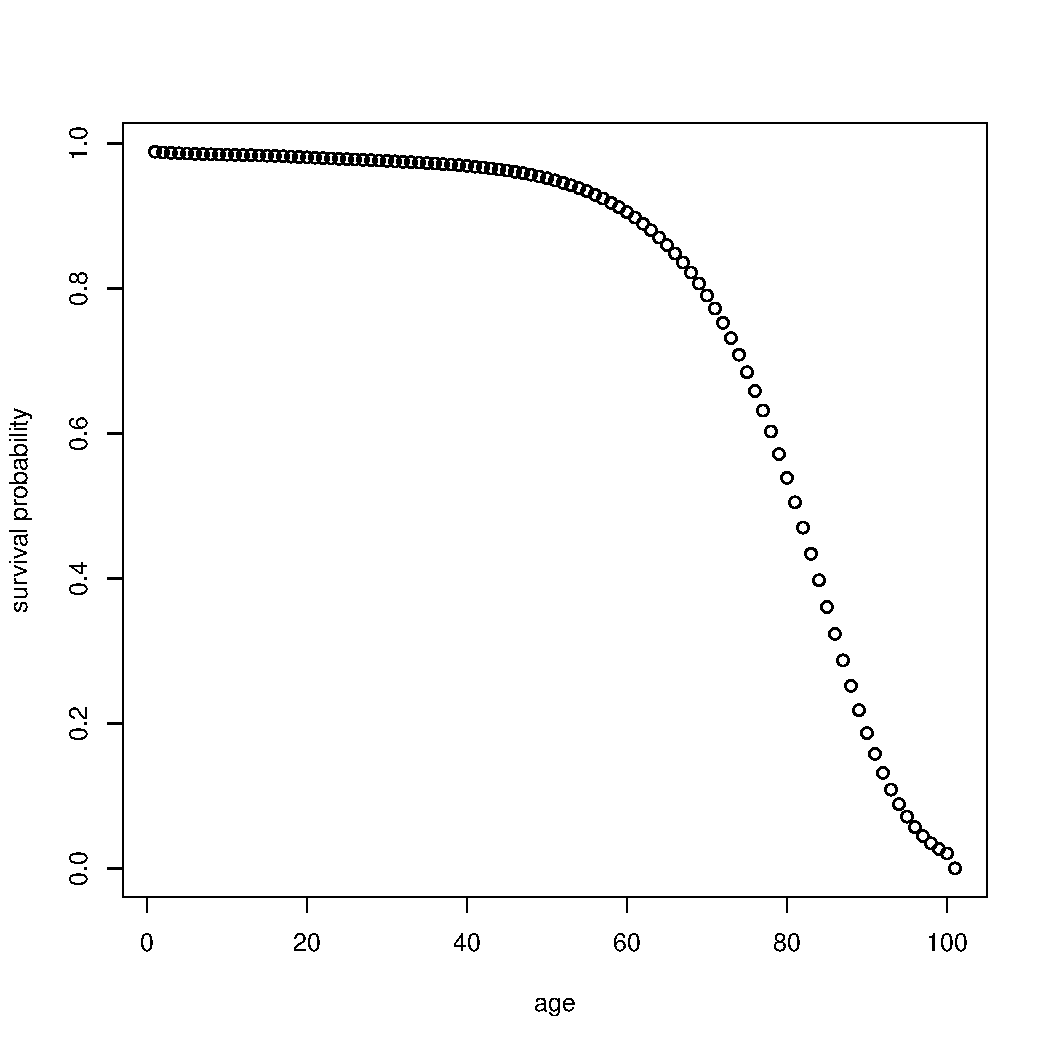
\includegraphics[scale=0.6]{figs/survival.pdf}
	\caption{Survival probabilities by age}
\end{figure}

\begin{table}
	\centering
	\caption{Benchmark Parameters}
	\begin{tabular}[c]{lll}
		\hline
		Parameter&Description&Value\\
		\hline
		$Y$&Beginning age&$28$\\
		$R$&Retirement age&$57$\\
		$T$&Lifespan (years)&$100$\\
		$\gamma$&Risk aversion&$5$\\
		$\beta$&Discount rate&$0.89$\\
		$r_f$&Risk-free rate&$0.108$\\
		$\pi$&Average inflation rate&$0.084$\\
		\hline
		$\mu_s$&Expected stock returns&$0.232$\\
		$\mu_h$&Expected housing returns&$0.113$\\
		$\sigma_s$&Stock returns volatility&$0.36$\\
		$\sigma_h$&Housing returns volatility&$0.052$\\
		$\sigma_w$&Wage growth volatility&$0.056$\\
		$\rho_{hs}$&Housing-stock correlation&$0.24$\\
		$\rho_{hw}$&Housing-wage correlation&$0.37$\\
		\hline
		$p_{28}$&Survival probability at age 28&$0.977$\\
		$p_{57}$&Survival probability at age 57&$0.924$\\
		$p_{100}$&Survival probability at age 100&$0$\\	
		\hline
	\end{tabular}
\end{table}


\subsubsection{Heterogeneity parameters}
In the same manner as Olear(2014) we will use wage growth rate, stock-income correlation and idiosyncratic labor income risk to model heterogeneities in education and sector. Let's now consider the heterogeneities one at a time:

\paragraph{Heterogeneity in education}
In line with Olear's (2016) approach we model the heterogeneity in education using the differences in wage growth rates. Indeed, we expect the salaries for higher education level to grow faster than for the lower education level. Some of this expectation comes from the fact that people with lower education are restricted in their career ladders and cannot rise very high in a workplace. Another intuition is that while college dropouts start working immediately, college graduates and graduate students continue to study and thus report zero income. When they graduate, their salary immediately rises from zero to the average salary, and this constitutes a steeper wage growth curve at the beginning of their lives. Figure 4.5 shows the wage series for different levels of education. Note that the curves for the lowest education levels are practically flat and the those for the highest education levels have varying non-zero slopes. 

\begin{figure}[h]
	\centering
	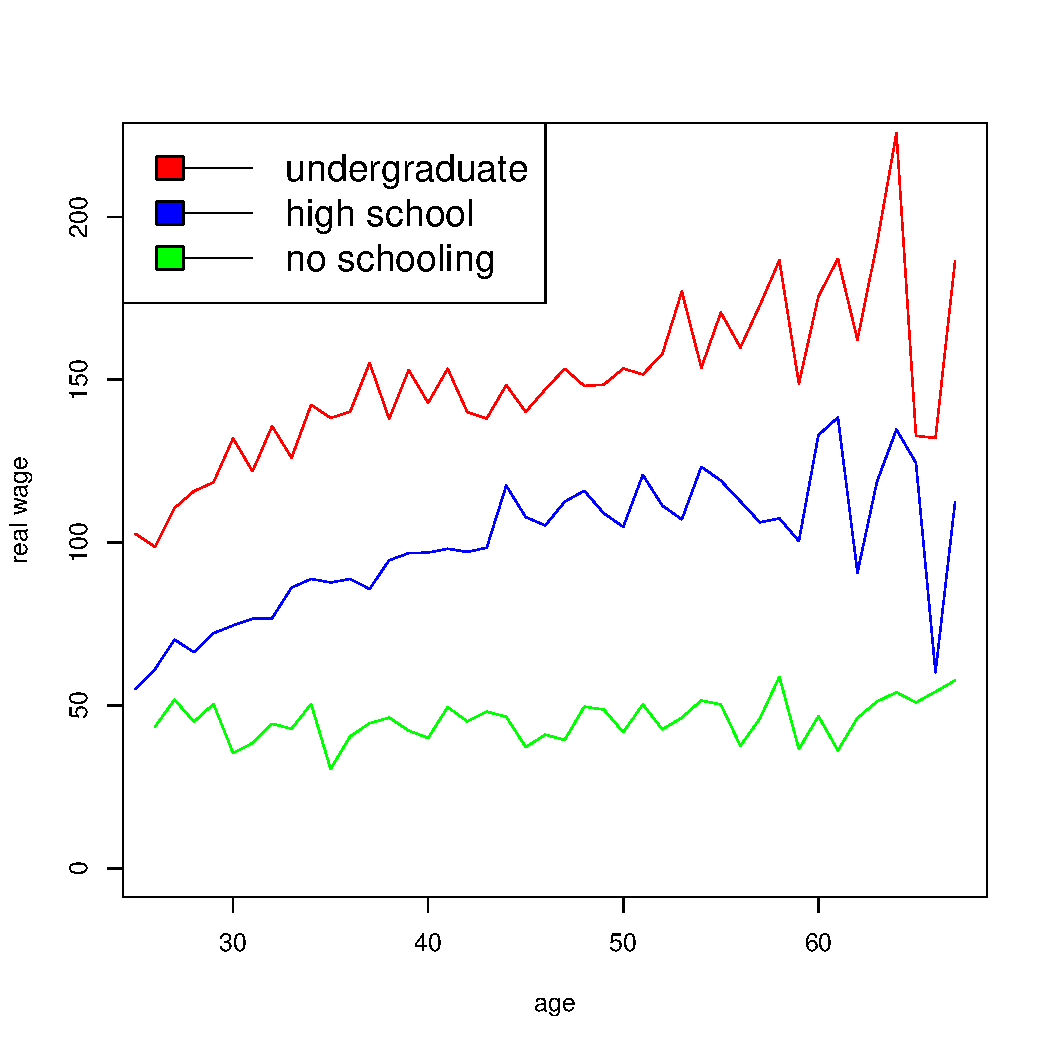
\includegraphics[scale=0.6]{figs/wage2educ.pdf}
	\caption{Lifetime wage dynamics by education level}
\end{figure}

Performing kinked regressions of log wages on ages, as described in the previous chapter, yielded best linear fits for three different education levels of our choice: postgraduate, high school, and no schooling. The corresponding labor income growth rates can be characterized as steep, moderate, and flat respectively. We considered wage data until 60 years, as Turkish retirement age is at 57, and have added empirically best kinks at ages 35 and 45. The results are summarized in Table 4.2 and illustrated in Figure 4.6. In this figure red lines represent the actual wages dynamics for postgraduate, high school, and no schooling, and blue lines are plots of the percentage changes proposed in Table 4.2, where the starting points all correspond to the actual starting points from the data. Figure 4.7 illustrates the same parameterized curves without actual wage curves. 

\begin{table}
	\centering
	\caption{Estimated Benchmark Wage Growth Rates $\mu_w$}
	\begin{tabular}[c]{l|ccc}
		Age&Flat&Moderate&Steep\\
		\hline
		0-35&0\%&3.5\%&6.5\%\\
		36-45&0\%&3\%&2\%\\
		46-60&0\%&0\%&0\%\\
	\end{tabular}
\end{table}


\begin{figure}[h]
	\centering
    \begin{minipage}{0.45\textwidth}
		\centering
		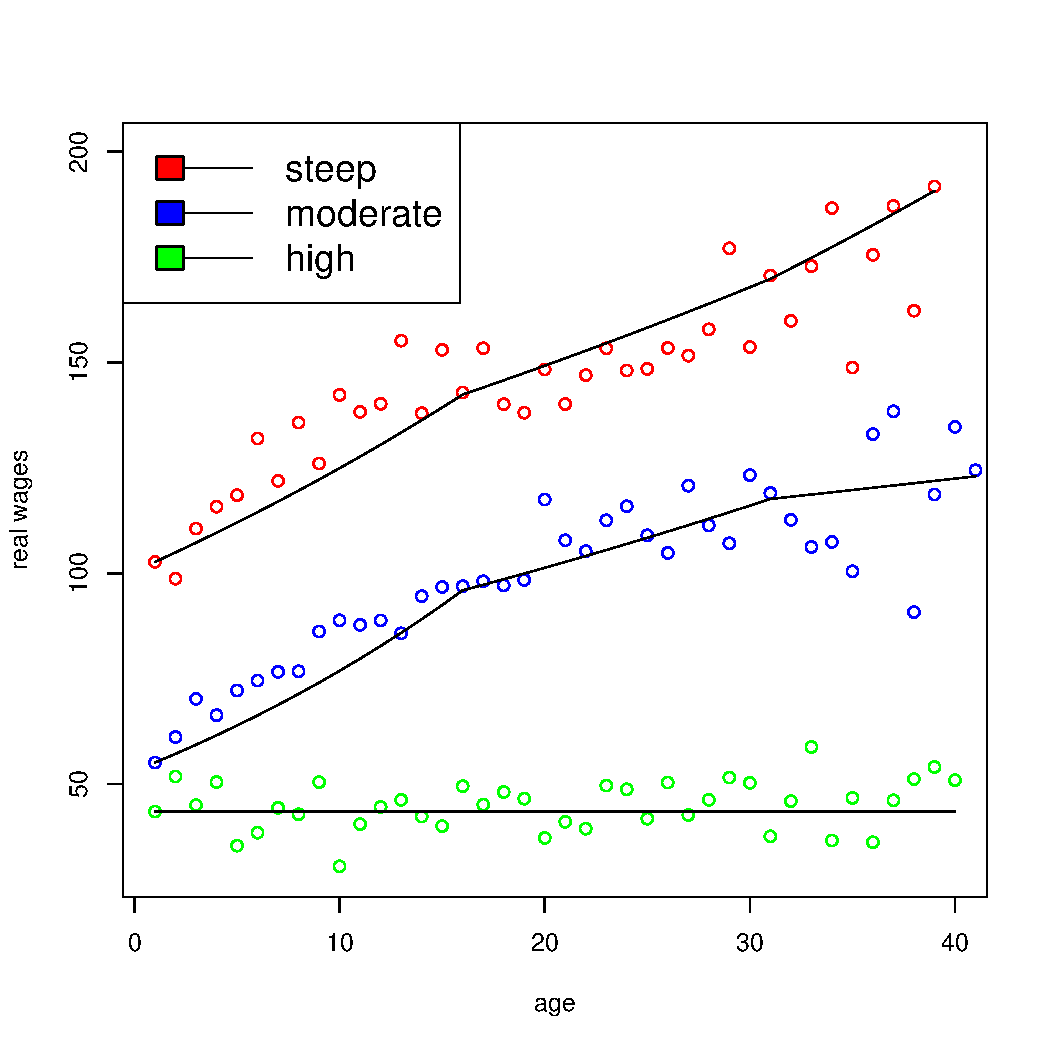
\includegraphics[scale=0.4]{figs/heterwage.pdf}
		\caption{Actual and parameterized benchmark wage dynamics by age}
	\end{minipage}
	\hfill
    \begin{minipage}{0.45\textwidth}
		\centering
		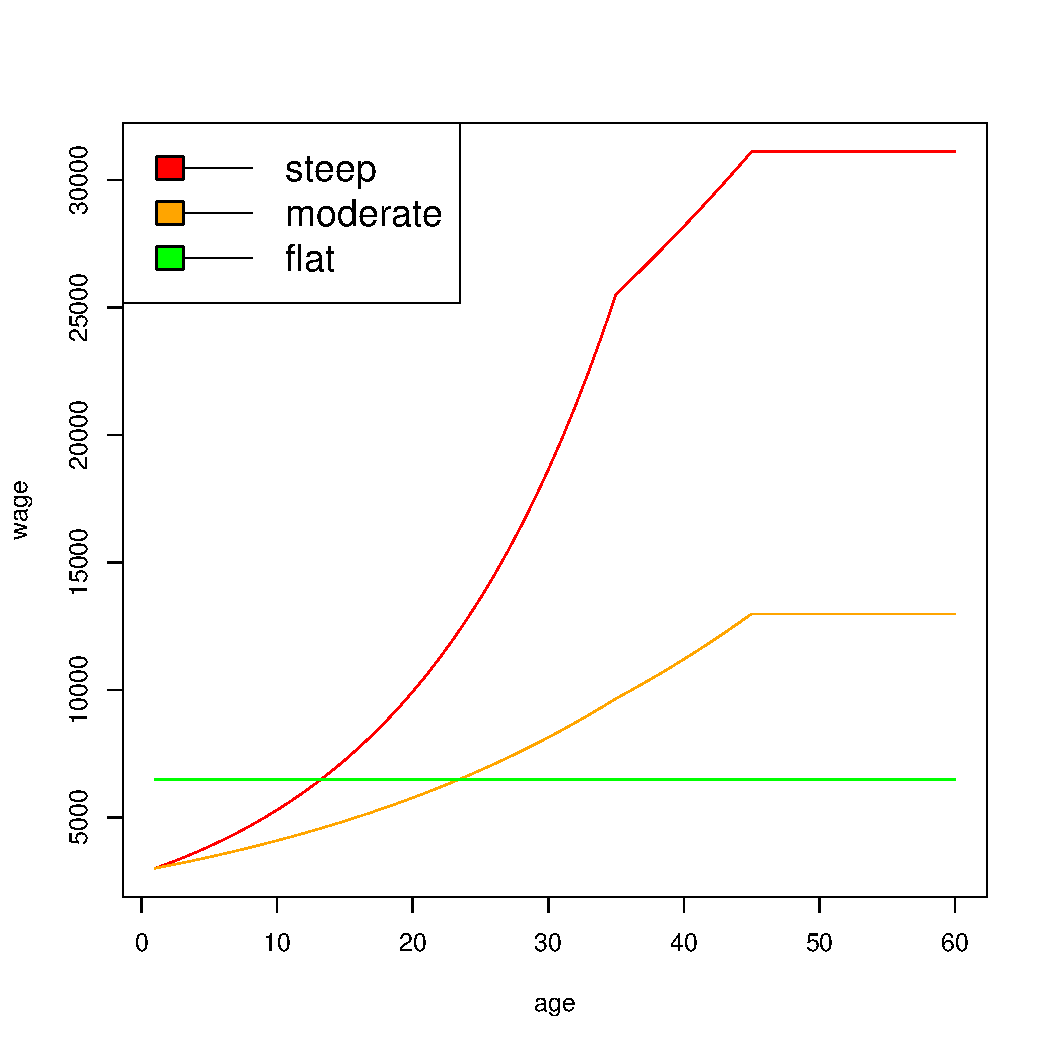
\includegraphics[scale=0.4]{figs/heterwageless.pdf}
		\caption{Parameterized wage dynamics by age}
	\end{minipage}

\end{figure}


\paragraph{Heterogeneity in sectors of work}

As we explained in Chapter 3, we model our labor income series as functions of age, gender, education, sector of work etc. We already showed in previous section how we incorporated the heterogeneity in education. We also stated at the beginning of this chapter that we consider only male individuals as heads of households; age is implicit in our analysis. In this section we will model the differences in sectors of work. Again, similar to Olear's (2016) approach we model these differences using correlations of wage growth rates with stock market returns. Indeed, it is expected that sectoral wages would be proportional to the stock returns only to the extent of their exposure to stock markets. In that sense, the stock-wage correlations are expected to be zero for public sector, where wages are fixed regardless the markets, and high in financial institutions. When we juxtaposed wages by sector and stock prices we obtained very high correlations, which was expected due to the economic growth over the years represented in Figure 4.8. Therefore we divided the wages by price levels to obtain the real wages, and, as expected, we obtained more realistic correlations. The financial sector's correlations were as high as $0.44$  and public sector, social service and education's were as low as $0.08$. Thus, our expectations that different sectors have different wage-stock correlation $\rho_{sw}$ were confirmed and we decided on three measures of $\rho_{sw}$ as our simulation benchmarks: $0$, $0.2$ and $0.4$ as stated in Table 4.3.

\begin{figure}[h]
	\centering
	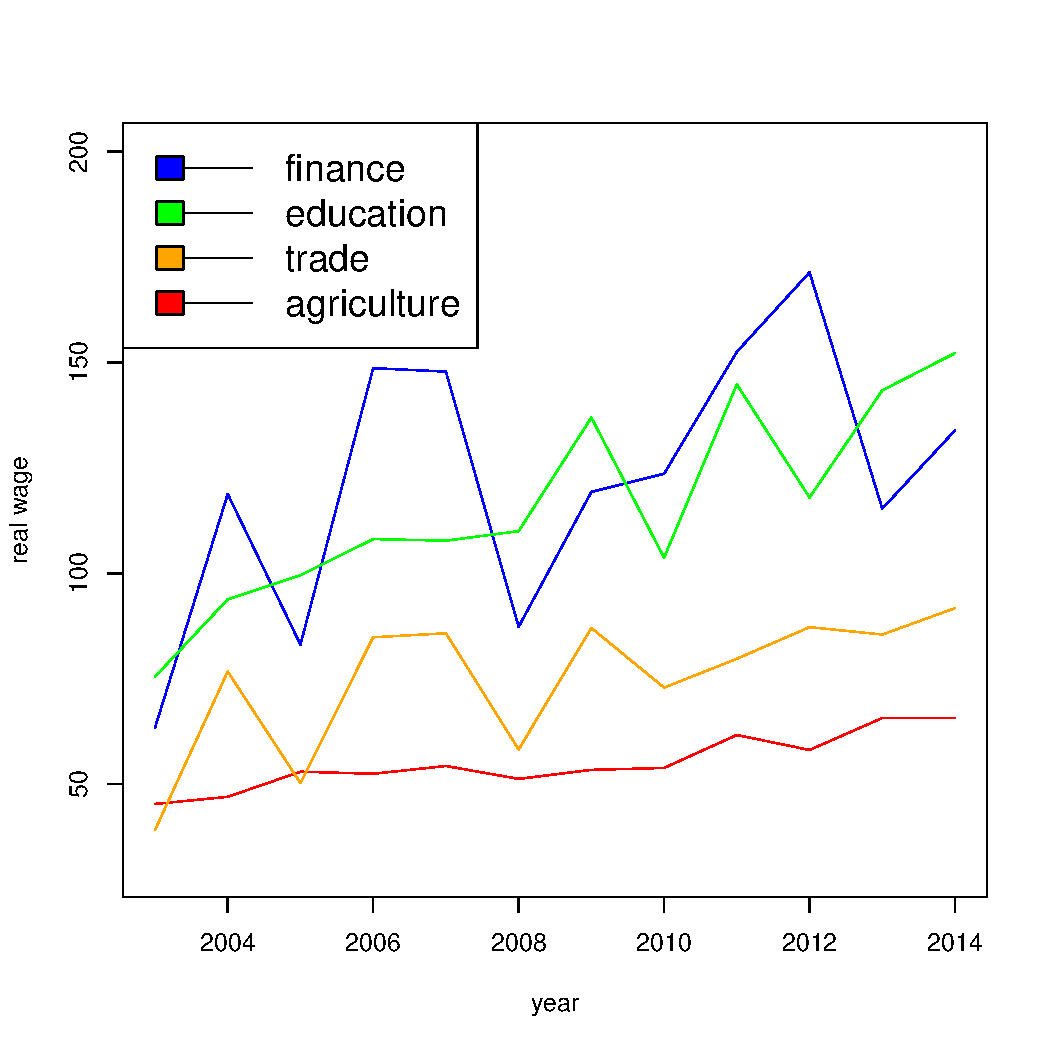
\includegraphics[scale=0.6]{figs/wage2sec.pdf}
	\caption{Historical wage dynamics by sector}
\end{figure}

\begin{table}
	\centering
	\caption{Benchmark Wage to Stock Correlations}
	\begin{tabular}[c]{c|ccc}
		&Low&Moderate&High\\
		\hline
		$\rho_{sw}$&0&0.2&0.4
	\end{tabular}
\end{table}


\paragraph{Individual heterogeneity}

%We model individual heterogeneity using idiosyncratic labor income shocks $\sigma_{\epsilon}$. We consider three different values $0.03$,$0.05$ and $0.07$. Total variance is calculated, as stated in previous chapter, as a sum of squares of aggregate and idiosyncratic shocks $\sigma^2_W = \sigma^2_w + \sigma^2_{\epsilon}$. This heterogeneity is summarized in Table 4.4. 


%\begin{table}
%	\centering
%	\caption{Benchmark Wage Volatilities and Their Sum of Squares}
%	\begin{tabular}[c]{l|ccc}
%		&Low&Moderate&High\\
%		\hline
%		$\sigma_w$&$0.056$&$0.056$&$0.056$\\
%		$\sigma_{\epsilon}$&$0.03$&$0.05$&$0.07$\\
%		\hline
%		$\sigma^2_{W}$&$0.004$&$0.0056$&$0.008$
%	\end{tabular}
%\end{table}

We check for individual heterogeneity using a sensitivity analysis on different risk aversion coefficients, summarized in Table 4.4.

\begin{table}
	\centering
	\caption{Coefficients of Risk Averion}
	\begin{tabular}[c]{r|cccc}
		Values&Torul&low&default&high\\
		\hline
		$\gamma$&1.5&3&5&10\\
	\end{tabular}
\end{table}

\subsection{Capital series}

\subsubsection{Human capital}
Human capital at all ages has been calculated as a discounted sum of all future wages until retirement with the discount factor $r_f$. To construct the individualized capital we used steep, moderate and flat wage series mentioned in the previous section. It can be seen in Figure 4.9 that human capital is declining for flat wages and hump-shaped for moderate and steep wages. 

\begin{figure}[h]
	\centering
    \begin{minipage}{0.45\textwidth}
		\centering
		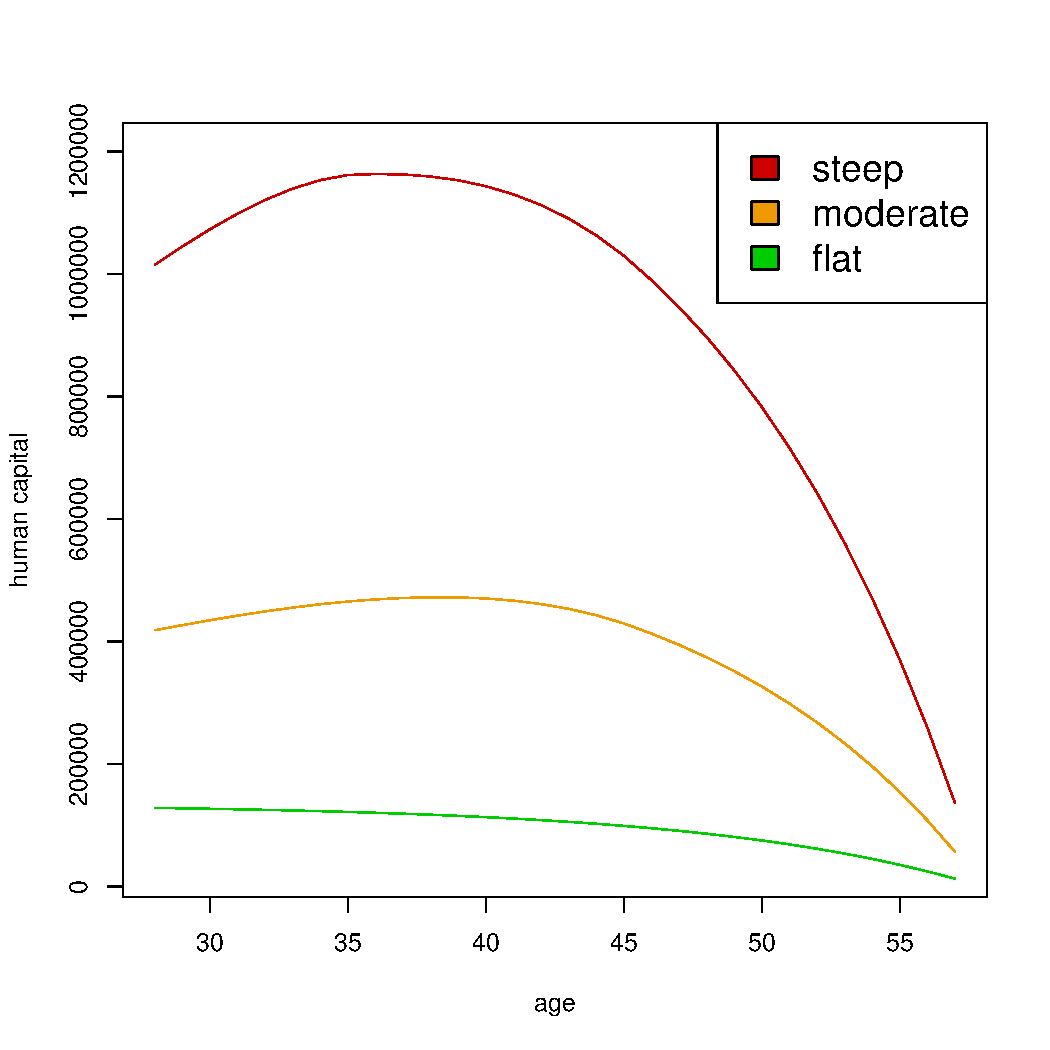
\includegraphics[scale=0.4]{figs/humancapital.pdf}
		\caption{Human capital by age}
	\end{minipage}
	\hfill
    \begin{minipage}{0.45\textwidth}
		\centering
		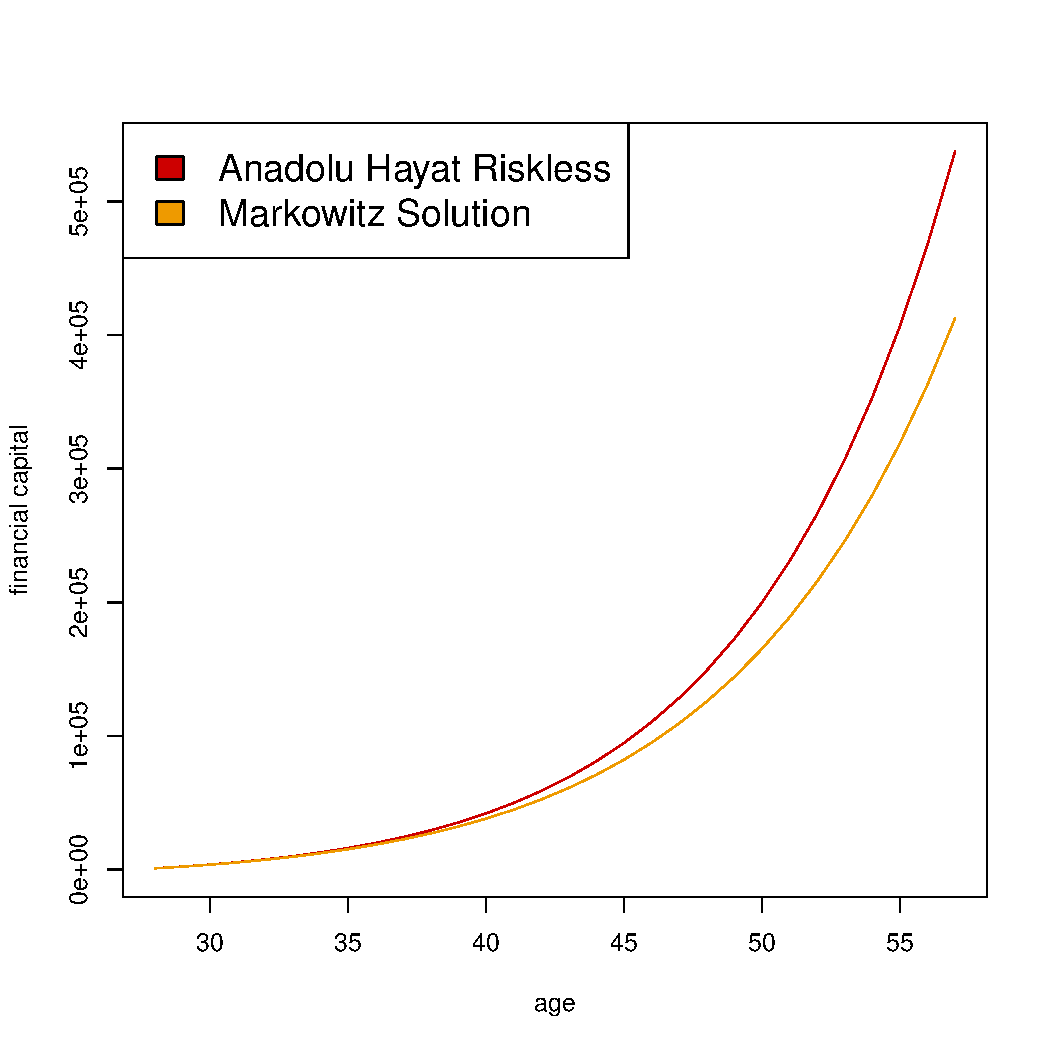
\includegraphics[scale=0.4]{figs/fincapital.pdf}
		\caption{Financial capital by age}
	\end{minipage}
\end{figure}

\subsubsection{Financial capital}

Financial capital evolves according to dynamic investment illustrated in Figure 4.11. Every period $t$ a certain percentage $c$ (equal to $3\%$ in Turkey) of that period's wage $w_t$ is invested in a retirement portfolio. At the same time, the previously invested amount accrues interest. We started with 28 years old individual who invests for 30 years until retirement, as has been mentioned previously numerous times.

\begin{figure}[h]
	\centering
	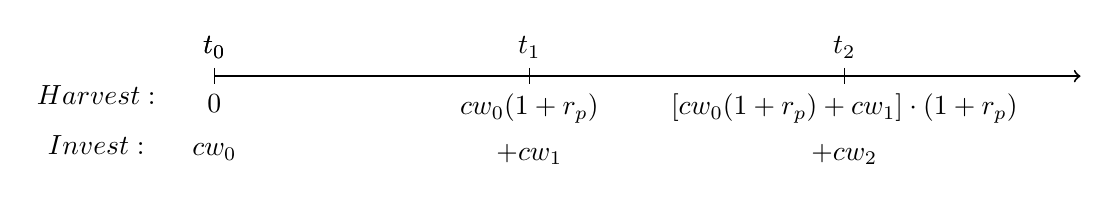
\begin{tikzpicture}
		\draw [->, line width=0.25mm] (0,0) -- (11,0);
		\foreach \x in {0,4,8}
			\draw (\x cm,3pt) -- (\x cm, -3pt);
		\draw (0,0) node[below=21pt] {$ cw_0 $} node[above=3pt] {$ t_0 $};
    	\draw (4,0) node[below=21pt] {$ +cw_1 $} node[above=3pt] {$ t_1 $};
    	\draw (8,0) node[below=21pt] {$ +cw_2 $} node[above=3pt] {$ t_2 $};
		\draw (0,0) node[below=3pt] {$ 0 $} node[above=3pt] {$ t_0 $};
    	\draw (4,0) node[below=3pt] {$ cw_0(1+r_p) $};
    	\draw (8,0) node[below=3pt] {$ \left[cw_0(1+r_p) + cw_1 \right] \cdot (1+r_p) $};
	    \draw (-1.5,0) node[below=18pt] {$ Invest: $};
    	\draw (-1.5,0) node[below=0pt] {$ Harvest: $};
	\end{tikzpicture}
	\caption{Law of motion of financial capital}
\end{figure}

\paragraph{}Note that the shape of the financial capital depends on $r_p$ --- the rate of return on portfolio, which itself depends on the risky-to-riskless asset ratio. Different such ratios are listed and analyzed in detail in the next section. Figure 4.10 demonstrates the evolution of financial capital for two investment options, provided by Anadolu Hayat Emeklilik --- $30\%$ in stocks and $70\%$ in bonds, and by solving Markowitz's formula --- $63\%$ in stocks and $37\%$ in bonds.

\paragraph{}It is important to notice here that since human capital is declining by age and financial capital is increasing, the ratio $\frac{L_t}{F_t}$ is declining in $t$. Recalling Merton's formula for $\alpha_t$ from Chapter 2, $\frac{\mu - R_f}{\gamma \sigma^2}(1+\frac{L_t}{F_t})$, it should be now clear how the above fraction creates a lifecycle effect --- different ratios for different ages. 


RESULTS HERE START In this chapter we present the results of our simulation. In the first section we will present the default and individualized lifecycle investment strategies, the former being provided by real retirement funds and the latter being solved by Merton and Munk. We will plug in the heterogeneous parameters, described in detail in the previous chapter. In the next section, we will calculate the resulting financial capital flows and compare their welfare effects using their expected utilities, as mentioned in Chapter 3. 

\subsection{Investment strategies}
\subsubsection{Default lifecyccles}
As was discussed in the previous chapter, our individual decides between investing in risky (stocks) or risk-free (bonds) assets. The default allocations for share of risky asset are given by:

\begin{itemize}
	\item $100-t$, for all $t$
	\item $\begin{cases} 100\%, & t<40\\(200-2.5t)\%, & t\in[40,57]\end{cases}$
	\item $63\%$, for all $t$
	\item $30\%$, for all $t$
\end{itemize}

where the latter two are Markowitz's solution and Anadolu Hayat's moderate investment option respectively. Since we are only interested in age span between 28 and 57, Figure 5.1 shows the risky asset share $\pi_t$ only for that interval. 

\begin{figure}[h]
	\centering
	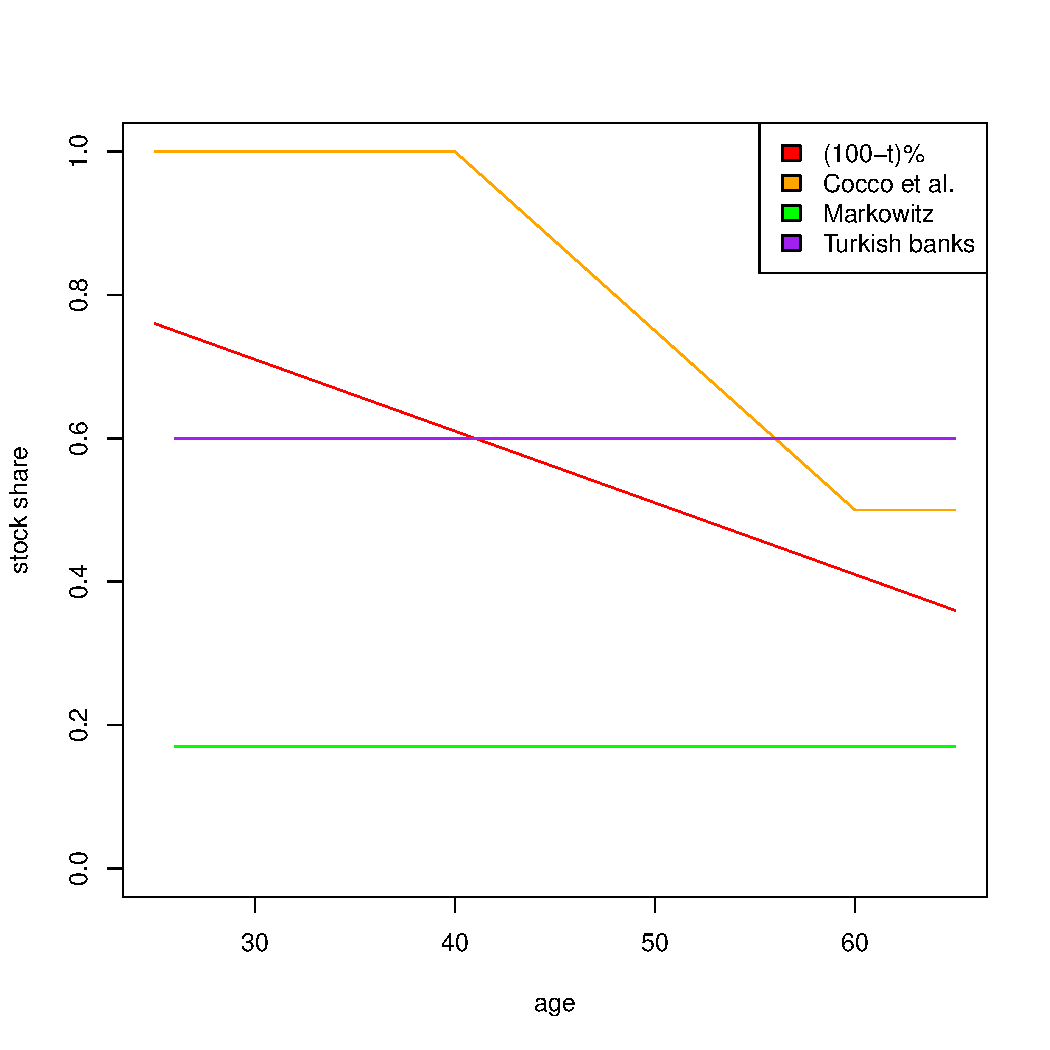
\includegraphics[scale=0.6]{figs/defaults.pdf}
	\caption{Default portfolio allocations of stock investments}
\end{figure}


\subsubsection{Individualized lifecycles}

To derive individualized lifecycle strategies, we used Merton's (1971) and Munk's (2016) optimal portfolio allocation formulas mentioned in chapters 2 and 3. Since these formulas depended on intratemporal amounts of capital, we have constructed three human capital series corresponding to flat, moderate and steep wage growth curves mentioned in the previous chapter. Figure 5.2 illustrates the risky asset shares given by Merton and Munk without housing for various levels of labor income growth and risk aversion. The figure shows that the steeper the wage growth curves get or the lower their risk aversion is, the more aggressive investors are. However, as a whole, they follow the similar pattern. The figure also shows that for small correlations between labor income and stock prices, Munk's solution converges to Merton's solution, as was shown in Chapter 3.

\begin{figure}
	\centering
    \begin{subfigure}{0.45\textwidth}
		\centering
		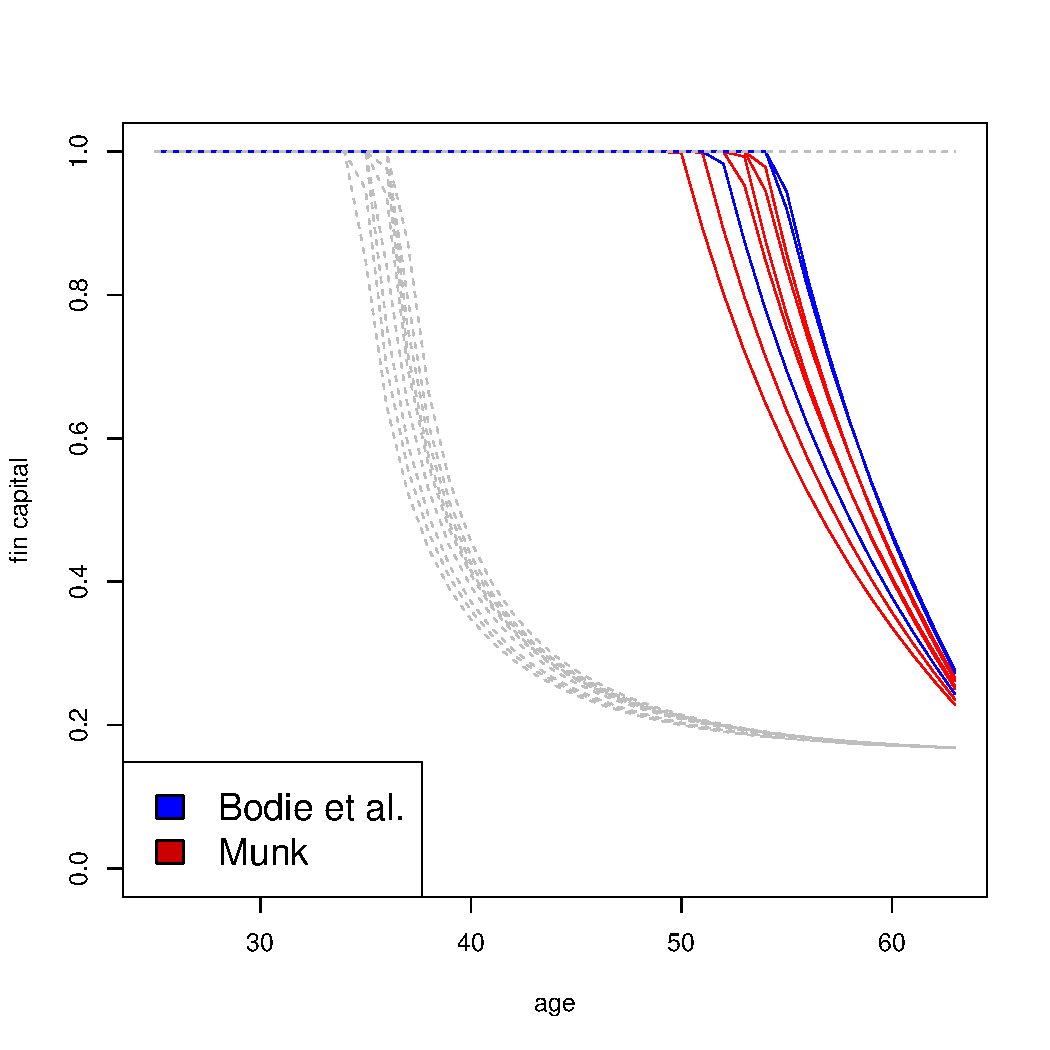
\includegraphics[scale=0.4]{figs/individuals15.pdf}
		\caption{$\gamma = 1.5$}
	\end{subfigure}
	\hfill
    \begin{subfigure}{0.45\textwidth}
		\centering
		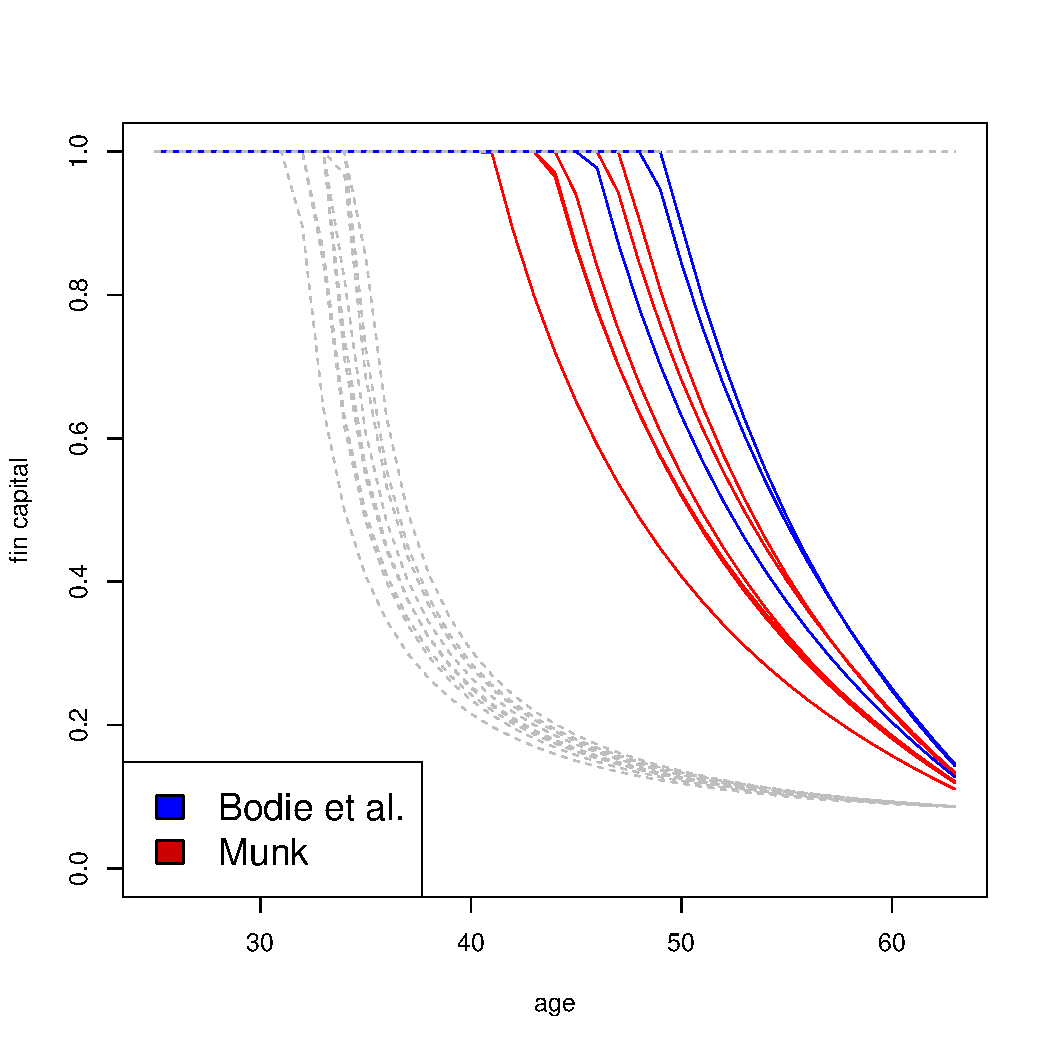
\includegraphics[scale=0.4]{figs/individuals3.pdf}
		\caption{$\gamma = 3$}
	\end{subfigure}
	\hfill
    \begin{subfigure}{0.45\textwidth}
		\centering
		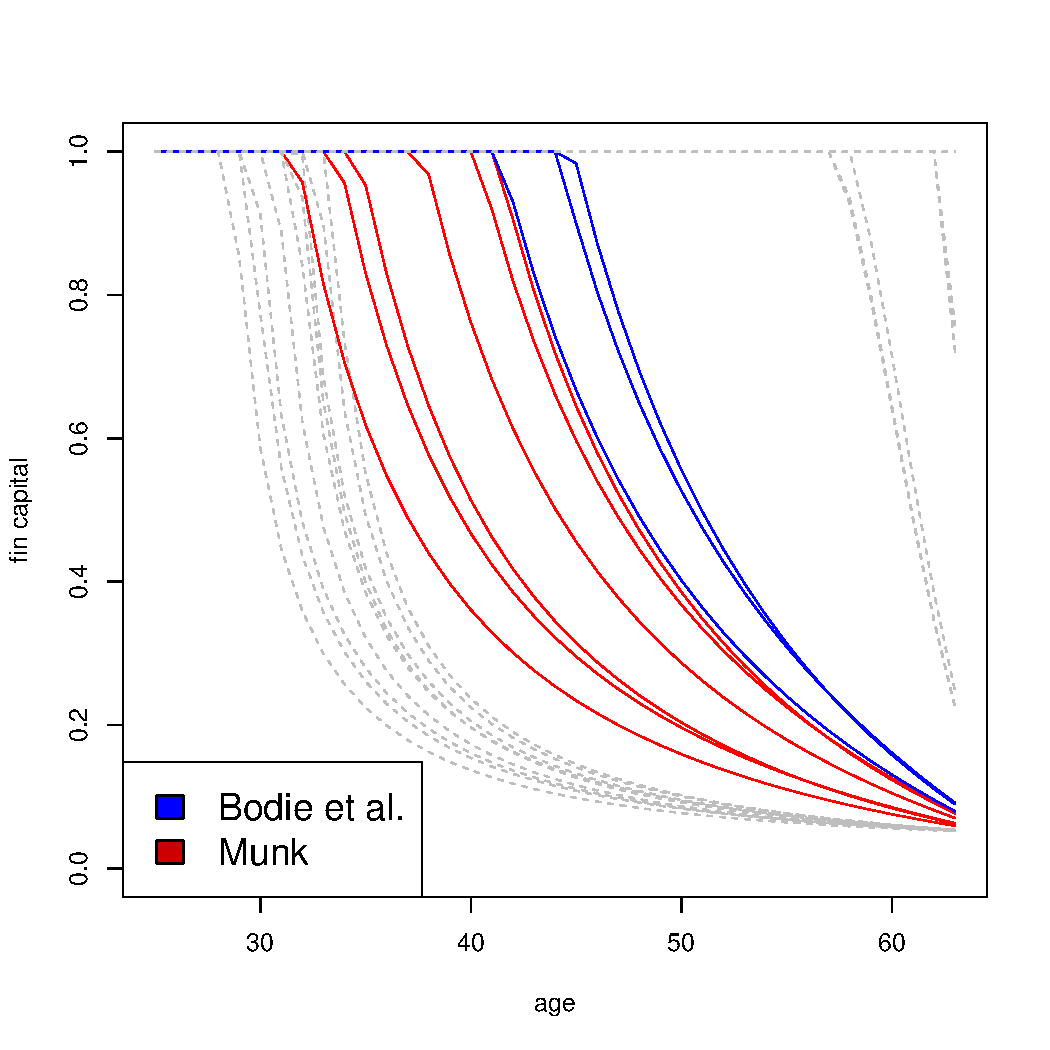
\includegraphics[scale=0.4]{figs/individuals5.pdf}
		\caption{$\gamma = 5$}
	\end{subfigure}
	\hfill
    \begin{subfigure}{0.45\textwidth}
		\centering
		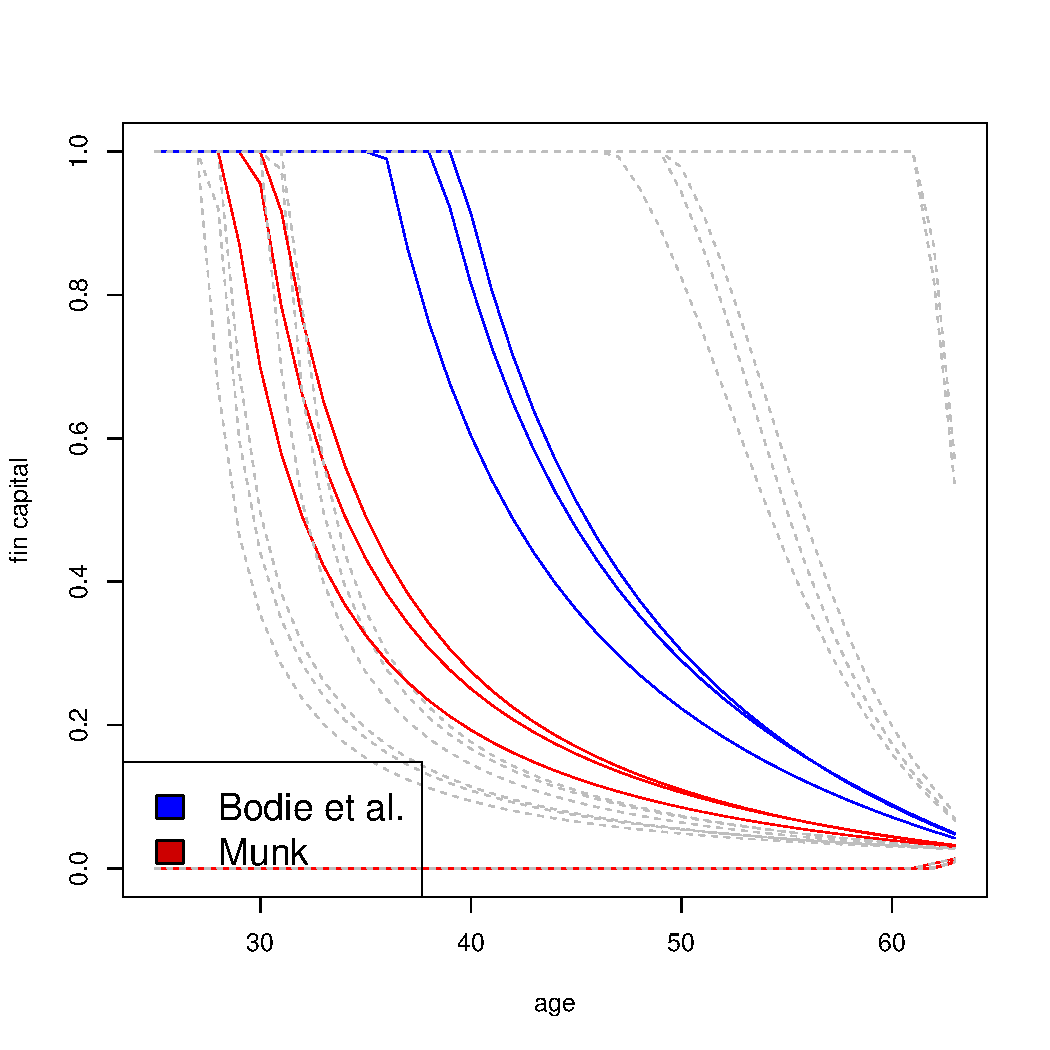
\includegraphics[scale=0.4]{figs/individuals10.pdf}
		\caption{$\gamma = 10$}
	\end{subfigure}
	\caption{Merton and Munk's solution without housing for different wage growth and risk aversion levels}
\end{figure}

\paragraph{}Figure 5.3 illustrates the stock and housing asset shares determined by Munk with housing for flat, moderate and steep labor income curves and low, moderate and high stock-labor income correlations for different levels of risk aversion, to capture heterogeneity, as mentioned in the previous chapter. The figure confirms that steeper labor income curves result in larger share of stocks in portfolio and less of bonds. Around age of 45, the sum of optimal stock and housing investments falls below $1$ and optimal bond investment becomes positive. Also, the higher the risk aversion, the less the individuals want to invest in both housing and stocks --- for $\gamma=10$, the optimal Munk solutions are negative or add up to less than $1$, meaning that they should sell all stocks and housing to invest in risk-free long term bonds. In our analysis we do not allow for negative investing, since this is not a primary focus of our thesis.  



\paragraph{}Full tables with actual solutions are available in Tables E.1 and E.2 of Appendix E for models without housing and in Table E.3 for a model with housing. 

% WELFARE COMPARISON
%%%%%%%%%%%%%%%%%%%%%%%%%%%%%%%%%%%%%%%%%%%%%%%%%%%%%%%%%%%%%%%%%%%%%%%%%%%%%%%%%%%%%%%%%%%%%%%%%%%%%%%%%%%%%%%%%%%%%%%%%%%%%%%%%%%%%
\section{Welfare comparison}
\label{welfare}

In order to compare welfare we use CRRA expected utility function, mentioned in Chapter 3. The probabilities of survival are taken from TUIK as mentioned in the previous chapter. The consumption is calculated in numbers of consumption baskets which cost exactly $1$ CPI --- consumer price index at that period, which is increasing with inflation rate annually, and is equal to $100$ at retirement age $57$. The wealth for which consumption baskets are purchased is a total accumulated wealth, including stock returns, bond returns and housing returns, annuitized according to the formula described in Chapter 3. Discount rate is $0.89$, as mentioned in the previous chapter. We compare expected utilities for different levels of risk aversion.

\begin{figure}[H]
	\centering
    \begin{subfigure}{0.45\textwidth}
		\centering
		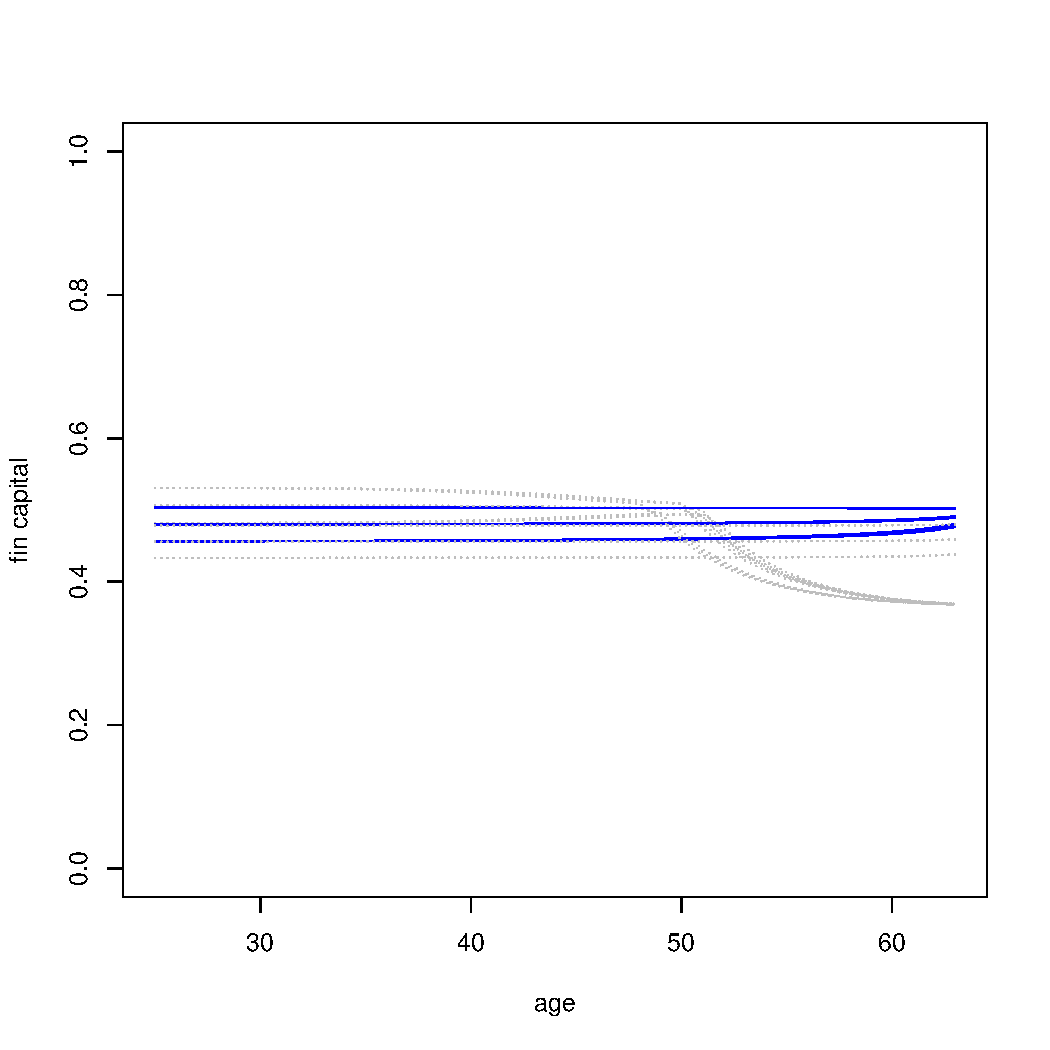
\includegraphics[scale=0.4]{figs/smunkhouse15.pdf}
		\caption{Stocks for $\gamma = 1.5$}
	\end{subfigure}
	\hfill
    \begin{subfigure}{0.45\textwidth}
		\centering
		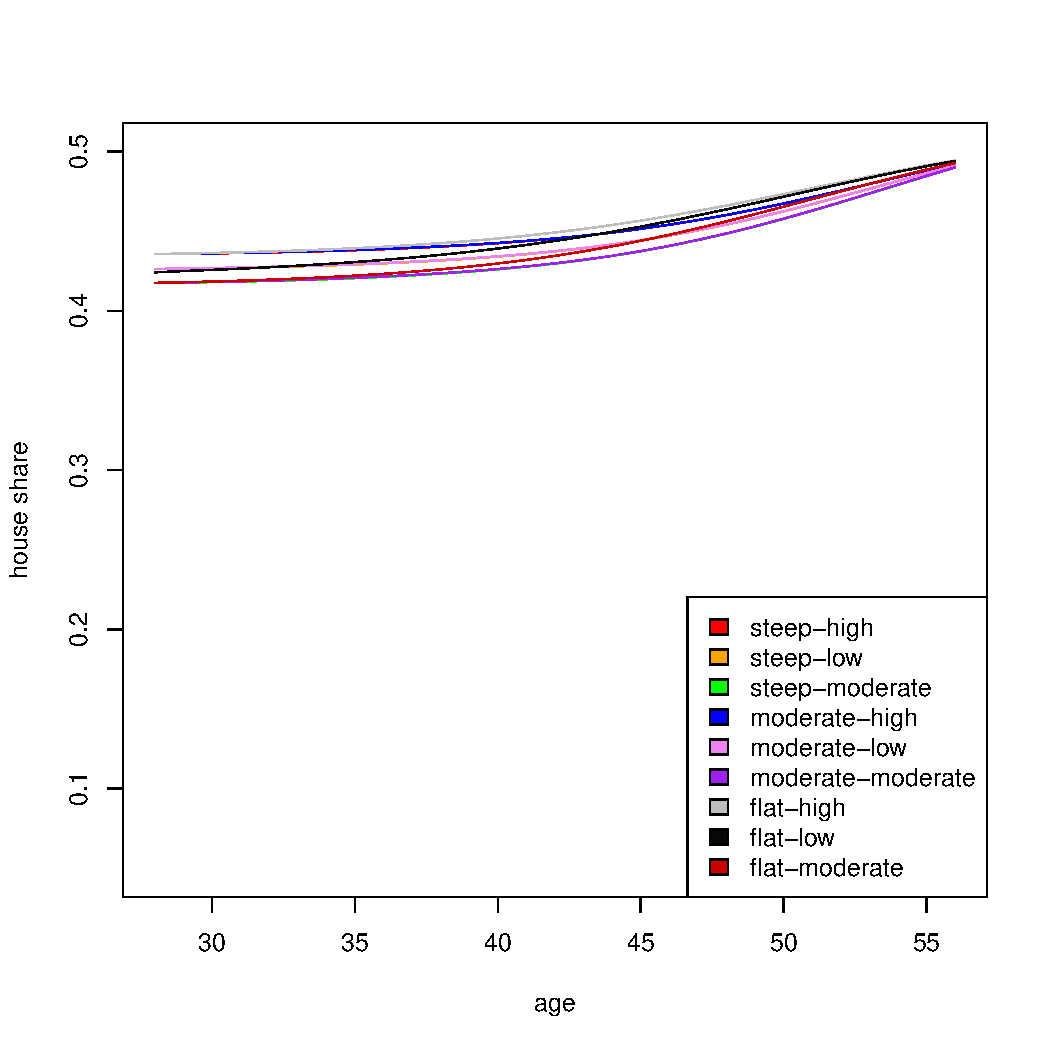
\includegraphics[scale=0.4]{figs/hmunkhouse15.pdf}
		\caption{Housing for $\gamma = 1.5$}
	\end{subfigure}
	\hfill
    \begin{subfigure}{0.45\textwidth}
		\centering
		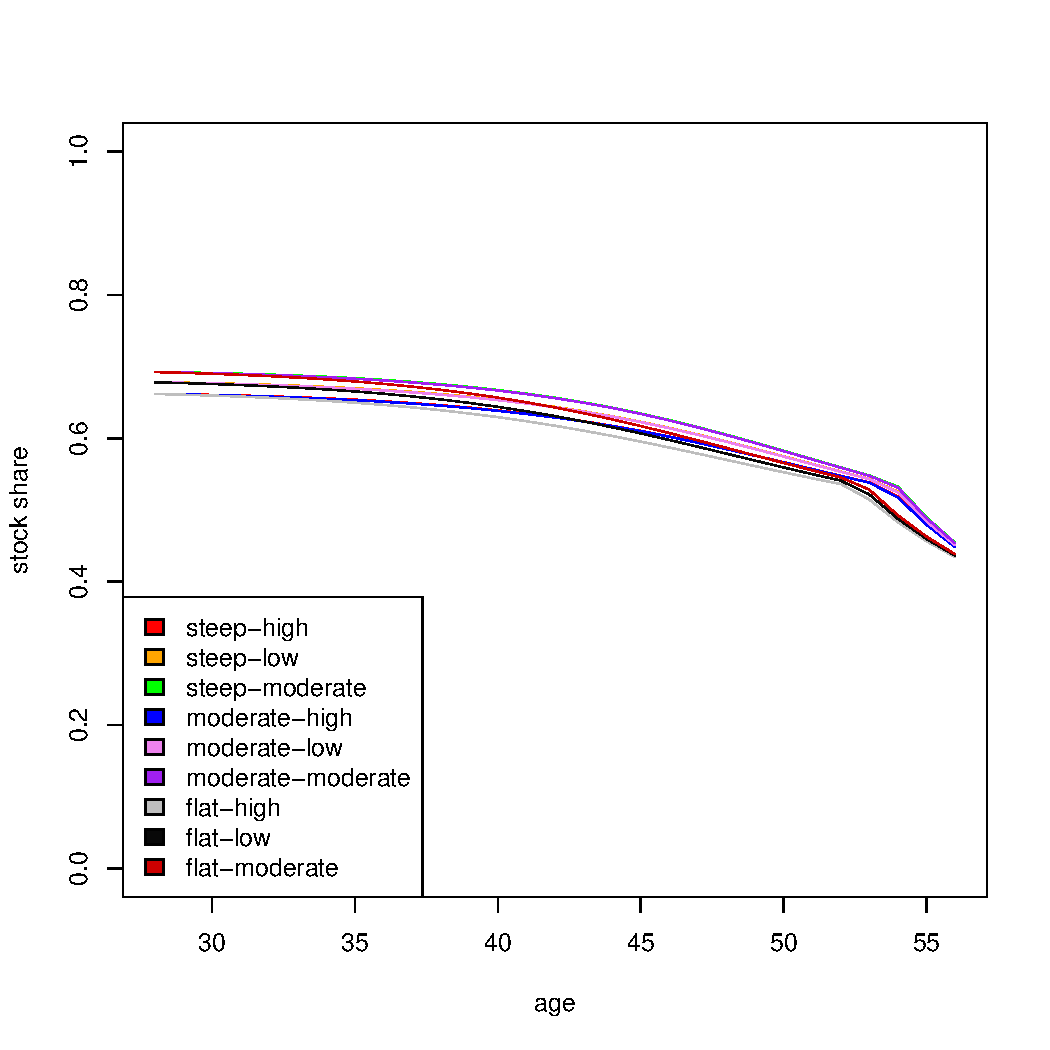
\includegraphics[scale=0.4]{figs/smunkhouse3.pdf}
		\caption{Stocks for $\gamma = 3$}
	\end{subfigure}
	\hfill
    \begin{subfigure}{0.45\textwidth}
		\centering
		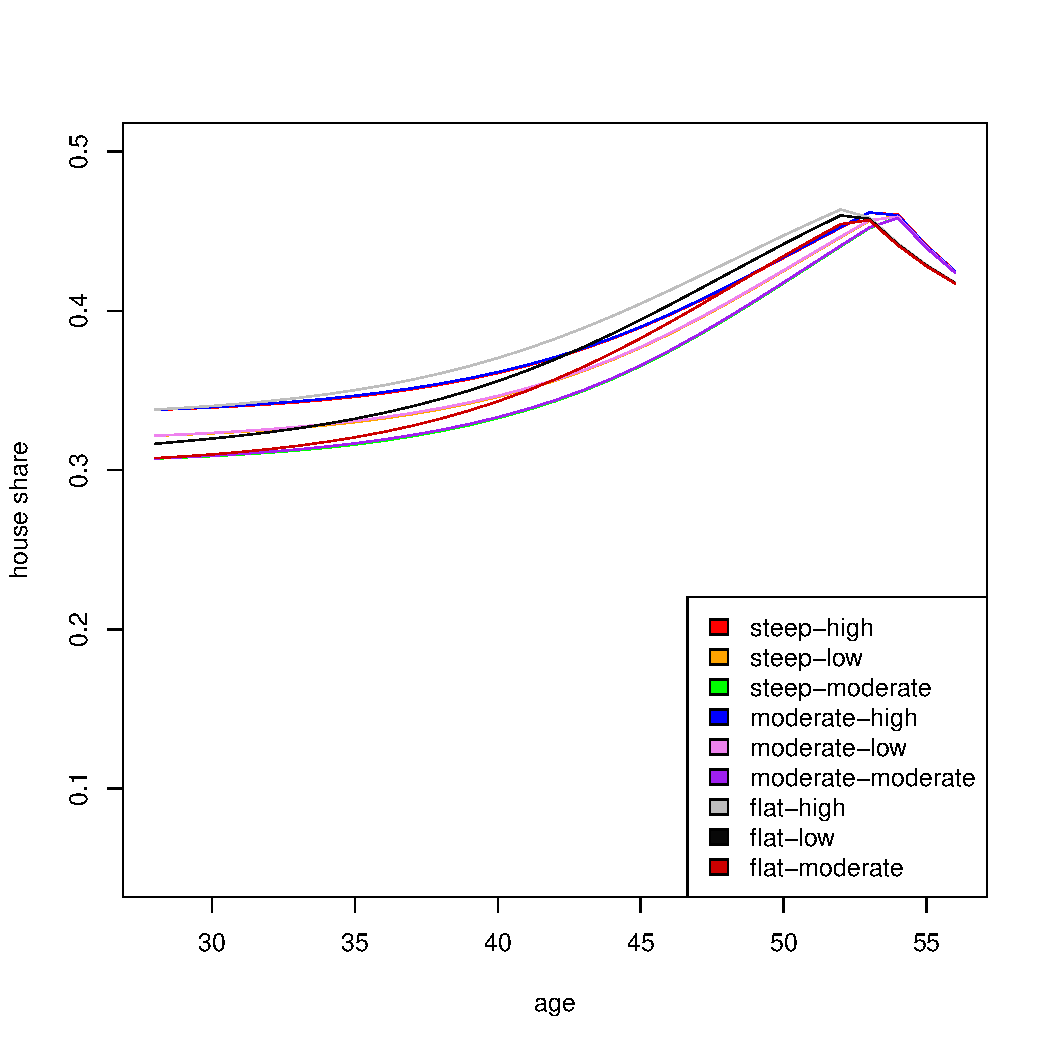
\includegraphics[scale=0.4]{figs/hmunkhouse3.pdf}
		\caption{Housing for $\gamma = 3$}
	\end{subfigure}
	\hfill
    \begin{subfigure}{0.45\textwidth}
		\centering
		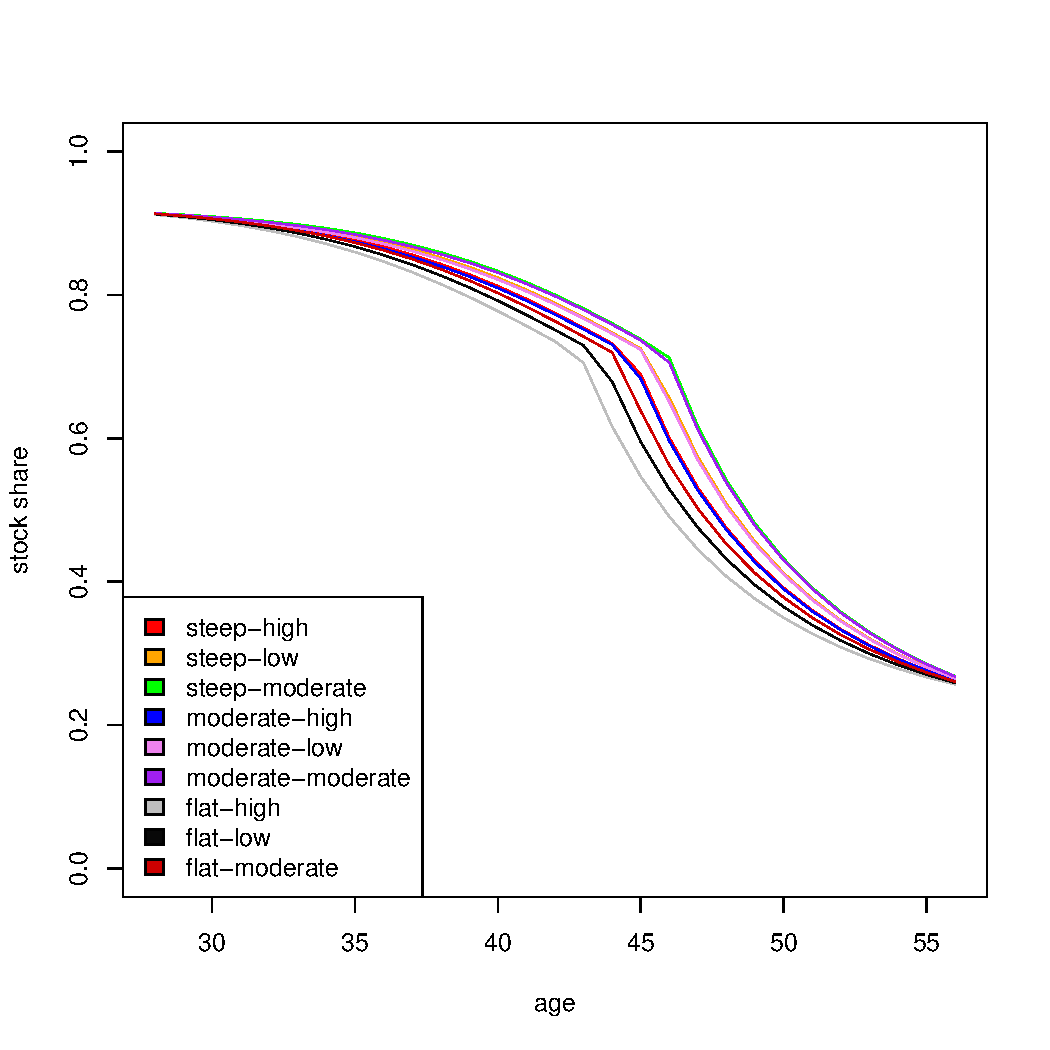
\includegraphics[scale=0.4]{figs/smunkhouse5.pdf}
		\caption{Stocks for $\gamma = 5$}
	\end{subfigure}
	\hfill
    \begin{subfigure}{0.45\textwidth}
		\centering
		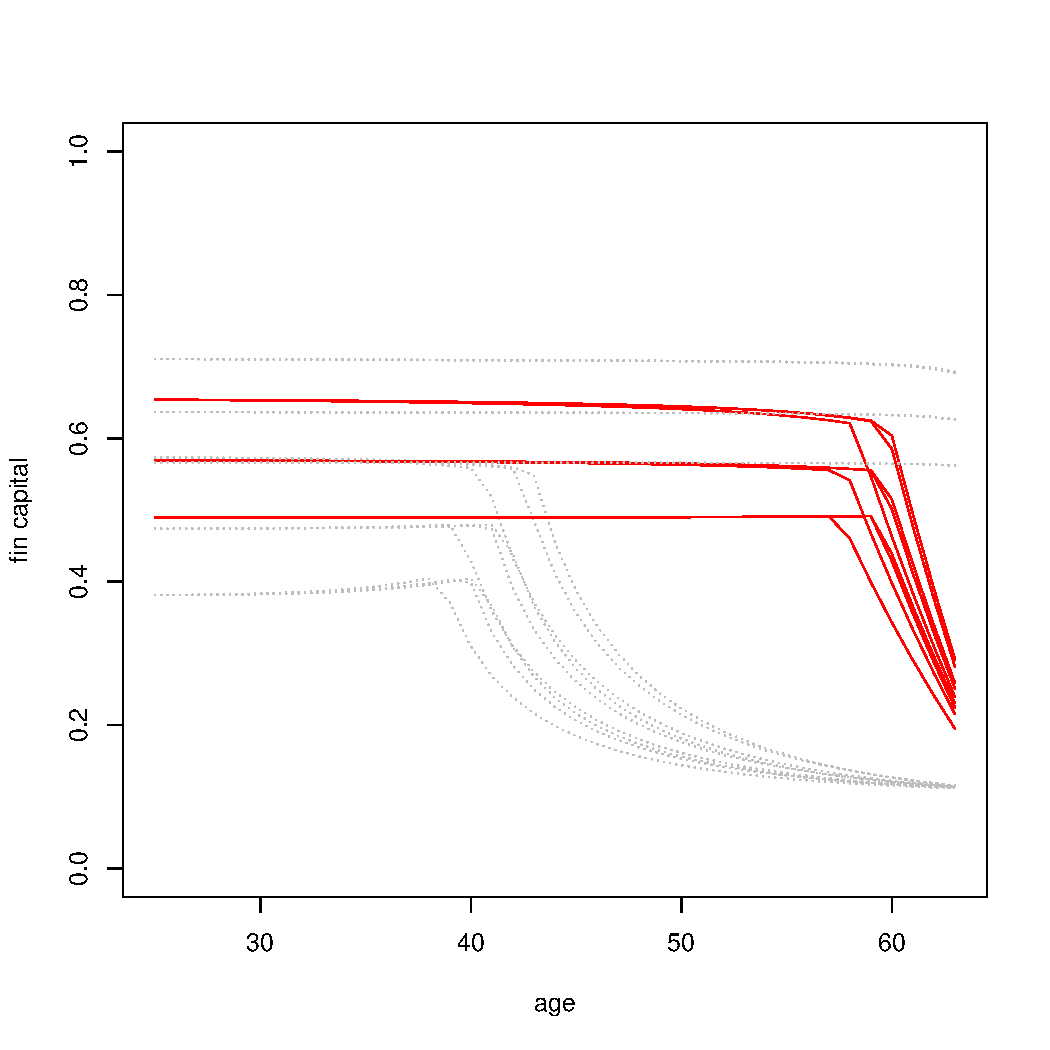
\includegraphics[scale=0.4]{figs/hmunkhouse5.pdf}
		\caption{Housing for $\gamma = 5$}
	\end{subfigure}
\end{figure}
\begin{figure}[H]\ContinuedFloat
    \begin{subfigure}{0.45\textwidth}
		\centering
		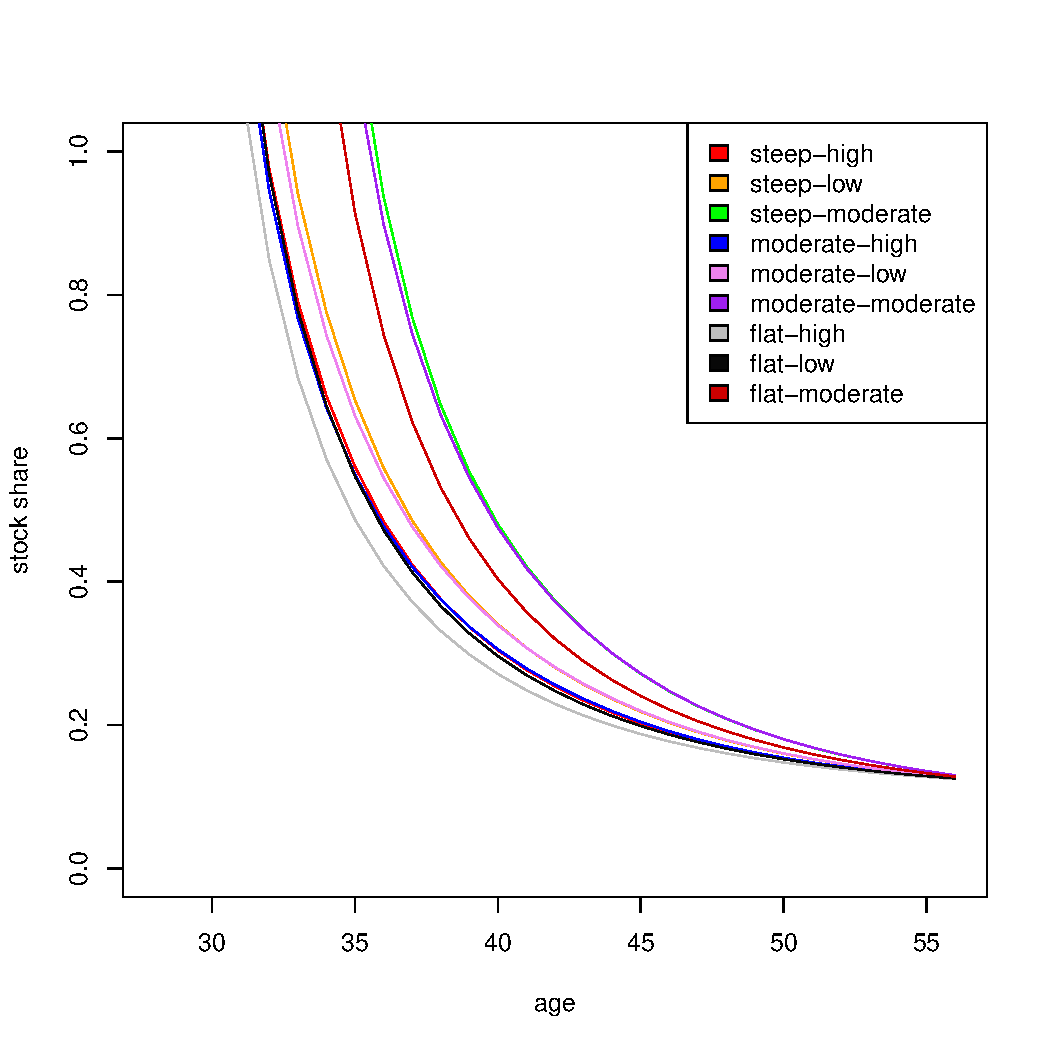
\includegraphics[scale=0.4]{figs/smunkhouse10.pdf}
		\caption{Stocks for $\gamma = 10$}
	\end{subfigure}
	\hfill
    \begin{subfigure}{0.45\textwidth}
		\centering
		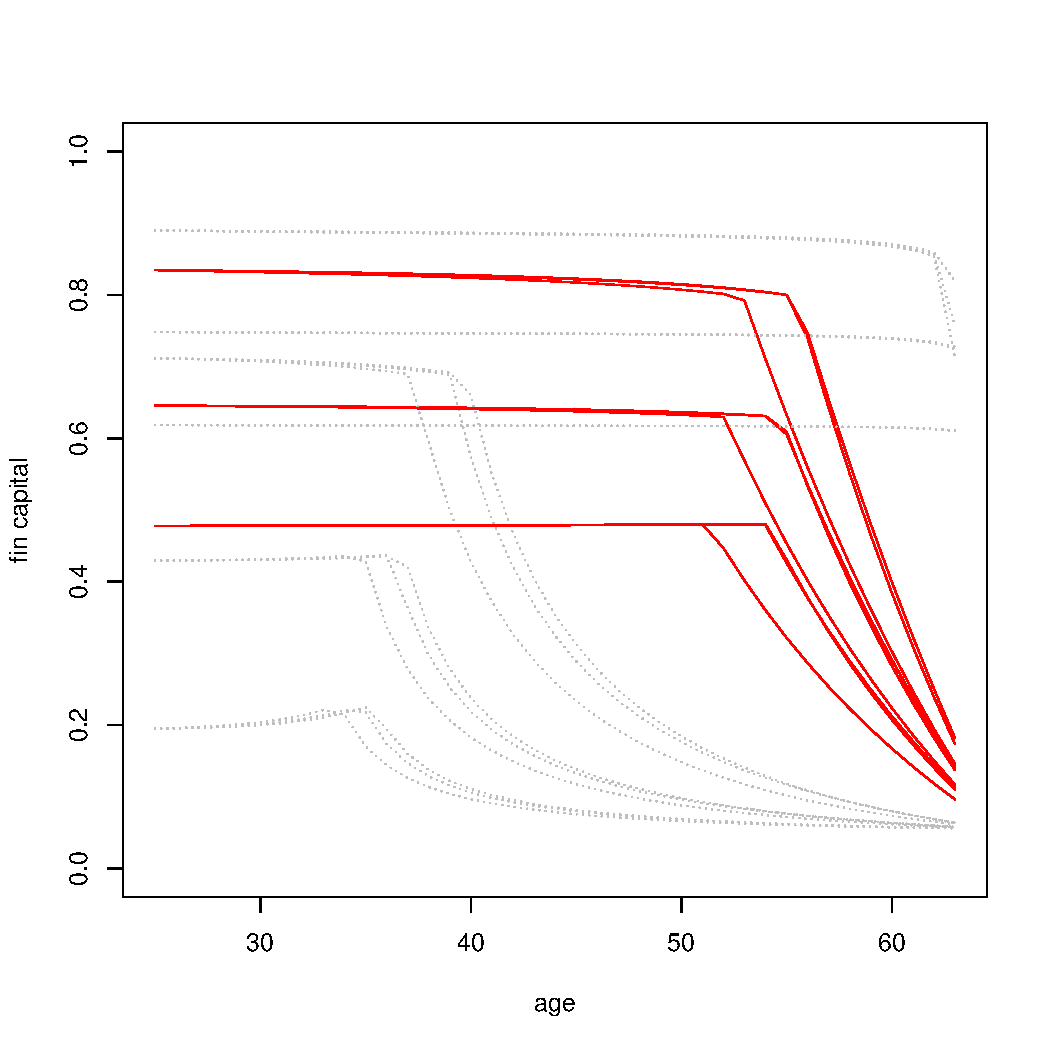
\includegraphics[scale=0.4]{figs/hmunkhouse10.pdf}
		\caption{Housing for $\gamma = 10$}
	\end{subfigure}
	\caption{Munk's stock and housing shares for different wage growth, stock-wage correlation and risk aversion levels}
\end{figure}

\subsubsection{Early results}

After a lifetime of investing in the above portfolios, the household accumulates different levels of wealth, summarized in Table 5.1. Since the consumption preferences are monotonic, we can make early conclusions even without calculating expected utilities --- the higher the accumulated wealth, the better: 

\begin{itemize}
\item Naively considering lifecycles does not guarantee the better investment. So, in our case, $(100-age)\%$ is worse than fixed Markowitz.
\item Different stock-wage correlations don't make much difference in the outcome without housing, and make considerable difference in models with housing
\item Stock-wage correlations are negatively correlated with total wealth
\item Both too low and too high risk aversion results in less accumulated capital than moderate risk aversion for models with housing and only too high risk aversion --- for models without housing (because of monotonicity).\\
\item Default options are better for people with flat wage growth rate and worse for people with moderate or steep wage curves
\end{itemize}

\subsubsection{Annuitization}
To formalize the observations made in the previous section, we will construct annuities and plug them into expected utility functions. As described in detail in Chapter 3, we define annuities by dividing the total wealth before retirement by the discount factor $1 + \sum^{100}_{t=58}\frac{p_t}{1+r_f}$. Using survival probabilities, obtained from TUIK, and risk-free rate of return, described in the previous chapter, we calculate the discount factor as $205.29$. The annuities are obtained by dividing all the values in the Table 5.1 by $205.29$. The resulting values are presented in Table 5.2. 


\subsubsection{Consumption during retirement}
We model that the individuals spend their annuity returns to consume baskets which cost $100$ TL during the year, when our agent is 58 years old, and increase by inflation rate $\pi = 8.4\%$. Thus, every period $t>57$ our agent consumes $\frac{annuity}{100\cdot\left(1.084\right)^{t-58}}$. We do not provide the separate table with the value streams, as they will be implicitly included in utility values.


\subsubsection{Expected utilities}
Finally, we will plug the consumption streams, calculated in the previous section, into the constant relative risk-aversion expected utility functions to compare the welfare effects. The resulting expected utility values are presented in Table 5.3.


\newgeometry{top=2cm,bottom=2cm}
\begin{table}%TABLE 5.1
	\centering
	\caption{Total Accumulated Wealth by Investment Option}
	\begin{tabular}[c]{lrrrr}
		\hline
		Option&$\gamma=5$ (default) & $\gamma=1.5$ & $\gamma=3$ & $\gamma=10$\\
		\hline
		\multicolumn{5}{c}{Defaults}\\
Anadolu Hayat (riskless)&614,195 TL&614,195 TL&614,195 TL&614,195 TL\\
$(100-age)\%$&1,160,977 TL&1,160,977 TL&1,160,977 TL&1,160,977 TL\\
Cocco et al.&1,599,852 TL&1,599,852 TL&1,599,852 TL&1,599,852 TL\\
Markowitz&1,300,187 TL&1,300,187 TL&1,300,187 TL&1,300,187 TL\\
\multicolumn{5}{c}{}\\
\multicolumn{5}{c}{Individualized (no housing)}\\
Merton (steep)&3,812,053 TL&4,212,735 TL&3,104,746 TL&2,920,892 TL\\
Merton (moderate)&1,629,904 TL&1,813,821 TL&1,447,951 TL&1,248,330 TL\\
Merton (flat)&543,602 TL&612,548 TL&639,866 TL&398,235 TL\\
Munk (steep-lo)&3,547,442 TL&4,168,823 TL&3,829,218 TL&2,085,883 TL\\
Munk (steep-mod)&3,543,435 TL&4,164,850 TL&3,825,221 TL&2,081,872 TL\\
Munk (steep-hi)&3,539,425 TL&4,160,872 TL&3,821,219 TL&2,077,854 TL\\
Munk (moderate-lo)&1,513,198 TL&1,794,772 TL&1,689,491 TL&868,955 TL\\
Munk (moderate-mod)&1,511,527 TL&1,793,113 TL&1,687,822 TL&867,281 TL\\
Munk (moderate-hi)&1,509,853 TL&1,791,452 TL&1,686,152 TL&865,604 TL\\
Munk (flat-lo)&508,757 TL&606,410 TL&657,762 TL&262,161 TL\\
Munk (flat-mod)&508,371 TL&606,025 TL&657,376 TL&261,774 TL\\
Munk (flat-hi)&507,984 TL&605,640 TL&656,990 TL&261,386 TL\\
\multicolumn{5}{c}{}\\
\multicolumn{5}{c}{Individualized (no housing)}\\
Munk (steep-lo)&8,937,159 TL&3,087,377 TL&4,718,332 TL&3,920,863 TL\\
Munk (steep-mod)&7,645,621 TL&2,966,467 TL&4,371,031 TL&2,900,022 TL\\
Munk (steep-hi)&6,353,327 TL&2,846,577 TL&4,017,054 TL&1,872,799 TL\\
Munk (moderate-lo)&3,652,223 TL&1,304,014 TL&1,998,234 TL&1,605,470 TL\\
Munk (moderate-mod)&3,125,930 TL&1,252,432 TL&1,850,278 TL&1,189,240 TL\\
Munk (moderate-hi)&2,599,301 TL&1,201,297 TL&1,700,235 TL&770,295 TL\\
Munk (flat-lo)&1,026,845 TL&430,353 TL&614,929 TL&455,296 TL\\
Munk (flat-mod)&881,934 TL&435,168 TL&598,789 TL&341,199 TL\\
Munk (flat-hi)&736,896 TL&397,829 TL&527,533 TL&226,188 TL\\
		\hline
	\end{tabular}
\end{table}
\resetgeometry


\newgeometry{top=2cm,bottom=2cm}
\begin{table}%TABLE 5.2
	\centering
	\caption{Annual Pensions by Investment Option}
	\begin{tabular}[c]{lrrrr}
		\hline
		Option&$\gamma=5$ (default) & $\gamma=1.5$ & $\gamma=3$ & $\gamma=10$\\
		\hline
		\multicolumn{5}{c}{Defaults}\\
Anadolu Hayat (riskless) TL&2,992 TL&2,992 TL&2,992 TL&2,992 TL\\
$(100-age)\%$ TL&5,655 TL&5,655 TL&5,655 TL&5,655 TL\\
Cocco et al. TL&7,793 TL&7,793 TL&7,793 TL&7,793 TL\\
Markowitz TL&6,333 TL&6,333 TL&6,333 TL&6,333 TL\\
\multicolumn{5}{c}{}\\
\multicolumn{5}{c}{Individualized (no housing)}\\
Merton (steep) TL&18,569 TL&20,521 TL&15,124 TL&14,228 TL\\
Merton (moderate) TL&7,940 TL&8,835 TL&7,053 TL&6,081 TL\\
Merton (flat) TL&2,648 TL&2,984 TL&3,117 TL&1,940 TL\\
Munk (steep-lo) TL&17,280 TL&20,307 TL&18,653 TL&10,161 TL\\
Munk (steep-mod) TL&17,261 TL&20,288 TL&18,633 TL&10,141 TL\\
Munk (steep-hi) TL&17,241 TL&20,268 TL&18,614 TL&10,122 TL\\
Munk (moderate-lo) TL&7,371 TL&8,743 TL&8,230 TL&4,233 TL\\
Munk (moderate-mod) TL&7,363 TL&8,735 TL&8,222 TL&4,225 TL\\
Munk (moderate-hi) TL&7,355 TL&8,726 TL&8,214 TL&4,216 TL\\
Munk (flat-lo) TL&2,478 TL&2,954 TL&3,204 TL&1,277 TL\\
Munk (flat-mod) TL&2,476 TL&2,952 TL&3,202 TL&1,275 TL\\
Munk (flat-hi) TL&2,474 TL&2,950 TL&3,200 TL&1,273 TL\\
\multicolumn{5}{c}{}\\
\multicolumn{5}{c}{Individualized (housing)}\\
Munk (steep-lo) TL&43,534 TL&15,039 TL&22,984 TL&19,099 TL\\
Munk (steep-mod) TL&37,243 TL&14,450 TL&21,292 TL&14,126 TL\\
Munk (steep-hi) TL&30,948 TL&13,866 TL&19,568 TL&9,123 TL\\
Munk (moderate-lo) TL&17,791 TL&6,352 TL&9,734 TL&7,820 TL\\
Munk (moderate-mod) TL&15,227 TL&6,101 TL&9,013 TL&5,793 TL\\
Munk (moderate-hi) TL&12,662 TL&5,852 TL&8,282 TL&3,752 TL\\
Munk (flat-lo) TL&5,002 TL&2,096 TL&2,995 TL&2,218 TL\\
Munk (flat-mod) TL&4,296 TL&2,120 TL&2,917 TL&1,662 TL\\
Munk (flat-hi) TL&3,590 TL&1,938 TL&2,570 TL&1,102 TL\\

		\hline
	\end{tabular}
\end{table}
\resetgeometry

\subsubsection{Conclusions}
Now, we can observe the final resutls:

\begin{itemize}

\item Naive lifecycle investment portfolios, such as $(100-age)\%$ don't overperform fixed-ratio Markowitz, because they don't take the risk aversion into consideration.
\item Cocco et al.'s $(200-2.5\cdot age)\%$ approximation is the best default portfolio. It is easy to interpret and captures lifecycle effect.
\item All models perform better for higher risk aversion and worse for lower risk aversion --- for everyone except flat-wagers.
\item Higher stock-wage correlation considerably decreases the utility for moderate and flat wages, and doesn't affect much for steep wages.
\item Merton's solution outperforms Munk's solution without housing for low levels of risk aversion, and performs same for high level of risk aversion ($\gamma=10$).
\item Munk's solution with housing outperforms every other solution for high levels of risk aversion ($\gamma=10$) --- for everyone except flat-wagers.
\item Munk's solution with housing outperforms Munk's solution without housing for $\gamma=5,10$.
\item Markowitz's solution outperforms both Merton's and Munk's solutions for flat wages and low risk aversion.
\item Individualizing lifecycles by wage growth rate and stock-wage correlation increases welfare for steep wagers and decreases welfare for flat wagers.
\end{itemize}

\paragraph{}We did not provide numerical conclusions, since they are trivial --- they can be obtained by calculating percentage differences in Table 5.3.

\newgeometry{top=2cm,bottom=2cm}
\begin{table}%TABLE 5.3
	\centering
	\caption{Expected Utilities by Investment Option}
	\begin{tabular}[c]{lrrrr}
		\hline
		Option&$\gamma=5$ (default) & $\gamma=1.5$ & $\gamma=3$ & $\gamma=10$\\
		\hline
\multicolumn{5}{c}{Defaults}\\
Anadolu Hayat (riskless)&-0.0008389&-3.6004130&-0.0247934&-0.0000509\\
(100-age)\%&-0.0000657&-2.6187470&-0.0069390&-0.0000002\\
Cocco et al.&-0.0000182&-2.2308240&-0.0036542&0.0000000\\
Markowitz&-0.0000418&-2.4745850&-0.0055327&-0.0000001\\
\multicolumn{5}{c}{}\\
\multicolumn{5}{c}{Individualized (no housing)}\\
Merton (steep)&-0.0000006&-1.3747480&-0.0009703&0.0000000\\
Merton (moderate)&-0.0000169&-2.0951160&-0.0044611&-0.0000001\\
Merton (flat)&-0.0013672&-3.6052480&-0.0228439&-0.0025138\\
Munk (steep-lo)&-0.0000008&-1.3819700&-0.0006379&0.0000000\\
Munk (steep-mod)&-0.0000008&-1.3826290&-0.0006392&0.0000000\\
Munk (steep-hi)&-0.0000008&-1.3832900&-0.0006405&0.0000000\\
Munk (moderate-lo)&-0.0000228&-2.1062050&-0.0032767&-0.0000022\\
Munk (moderate-mod)&-0.0000229&-2.1071790&-0.0032832&-0.0000023\\
Munk (moderate-hi)&-0.0000230&-2.1081550&-0.0032897&-0.0000023\\
Munk (flat-lo)&-0.0017820&-3.6234500&-0.0216177&-0.1082611\\
Munk (flat-mod)&-0.0017874&-3.6245990&-0.0216431&-0.1097095\\
Munk (flat-hi)&-0.0017929&-3.6257500&-0.0216686&-0.1111816\\
\multicolumn{5}{c}{}\\
\multicolumn{5}{c}{Individualized (housing)}\\
Munk (steep-lo)&0.0000000&-1.6058700&-0.0004201&0.0000000\\
Munk (steep-mod)&0.0000000&-1.6382700&-0.0004895&0.0000000\\
Munk (steep-hi)&-0.0000001&-1.6724140&-0.0005796&0.0000000\\
Munk (moderate-lo)&-0.0000007&-2.4709510&-0.0023424&0.0000000\\
Munk (moderate-mod)&-0.0000013&-2.5213210&-0.0027320&-0.0000001\\
Munk (moderate-hi)&-0.0000026&-2.5744240&-0.0032354&-0.0000066\\
Munk (flat-lo)&-0.0001074&-4.3012340&-0.0247341&-0.0007532\\
Munk (flat-mod)&-0.0001973&-4.2773710&-0.0260855&-0.0101044\\
Munk (flat-hi)&-0.0004049&-4.4735990&-0.0336084&-0.4086488\\

		\hline
	\end{tabular}
\end{table}
\resetgeometry

% CONCLUSION 
%%%%%%%%%%%%%%%%%%%%%%%%%%%%%%%%%%%%%%%%%%%%%%%%%%%%%%%%%%%%%%%%%%%%%%%%%%%%%%%%%%%%%%%%%%%%%%%%%%%%%%%%%%%%%%%%%%%%%%%%%%%%%%%%%%%%%

\section{Conclusion}
\label{conclusion}

In this thesis we have reviewed the current state of pension investments in Turkey and the history and recent developments of a field of financial economics. We have reviewed the concept of "lifecycle investment" and summarized the common models and heuristics.

\paragraph{}We have presented our model as an application of Munk's (2016) recent findings and Olear's (2016) simulation techniques into Turkish retirement market. We have collected historical data to calibrate and estimate the best parameters to be used in our simulation.

\paragraph{}Using these parameters, we have constructed heterogeneous agents, who worked and invested throughout their lifetime. We considered different investment models that our hypothetical agents would use and calculated the resulting investment capitals.

\paragraph{}Finally, we have calculated and compared the welfare effects of all popular models to the individualized Munk's solutions. We have concluded that for rich-to-middle class citizens, the individiualized strategies considerably increase their welfare. Moreover, the solutions we proposed can be solved analytically without complex dynamic optimizations, and therefore are easy to interpret to households. We also found that even naive lifecycle investments perform better than fixed lifetime investment.

\paragraph{}We propose these models to Turkish pension providers and to Turkish working-age households belonging to middle-to-upper class, as these options will increase their retirement welfare considerably.



% BIBLIOGRAPHY
%%%%%%%%%%%%%%%%%%%%%%%%%%%%%%%%%%%%%%%%%%%%%%%%%%%%%%%%%%%%%%%%%%%%%%%%%%%%%%%%%%%%%%%%%%%%%%%%%%%%%%%%%%%%%%%%%%%%%%%%%%%%%%%%%%%%%
\section{References}
\begin{thebibliography}{}
\bibitem[Markowitz(1952)]{markowitz} Markowitz H. (1952). Portfolio Selection. \textit{The Journal of Finance}, 7(1), 77-91.
\bibitem[Tobin(1958)]{tobin} Tobin J.(1958). Liquidity Preference as Behavior Towards Risk. \textit{The Review of Economic Studies}, 25(2), 65-86.
\bibitem[Merton(1971)]{merton} Merton R.C. (1971). Optimum Consumption and Portfolio Rules in a Continuous-Time Model. \textit{Journal of Economic Theory}, 3, 373-413.
\bibitem[Samuelson(1969)]{samuelson} Samuelson, Paul A. (1969). Lifetime Portfolio Selection by Dynamic Stochastic Programming. \textit{Review of Economics and Statistics}, 51(3), 239-246.
\bibitem[Canner et al.(1994)]{canner} Canner, N., Mankiw, N.G., Weil, D.N. (1997). An Asset Allocation Puzzle. \textit{The American Economic Review}, 87(1), 181-191.
\bibitem[Bodie et al.(1992)]{bodie}Bodie, Z., Merton, R.C., Samuelson, W.F. (1992). Labor Supply Flexibility and Portfolio Choice in a Life-Cycle Model. \textit{Journal of Economic Dynamics and Control}, 16(3-4), 427-449. 
\bibitem[Cocco et al.(2005)]{cgm} Cocco, J.F., Gomes, F.J., Maenhout P.J. (2005). Consumption and Portfolio Choice over the Life Cycle. \textit{The Review of Financial Studies}, 18(2), 491-533. 
\bibitem[Chang et al.(2014)]{chang} Chang, Y., Hong, J.H., Karabarbounis, M. (2014). Labor-Market Uncertainty and Portfolio Choice Puzzles. \textit{Working Papers, Federal Reserve Bank of Richmond}, 14(13).
\bibitem[Cocco(2004)]{cocco} Cocco, J.F. (2004). Portfolio Choice in the Presence of Housing. \textit{The Review of Financial Studies}, 18(2), 537-567.
\bibitem[Flavin and Yamashita(2002)]{flavin} Flavin M., Yamashita T. (2002). Owner-Occupied Housing and the Composition of the Household Portfolio. \textit{The American Economic Review}, 1, 345-362.
\bibitem[Munk(2016)]{munk} Munk C. (2016). A Mean-Variance Benchmark for Household Portfolios over the Life Cycle. \textit{Working Papers, Copenhagen Business School, Department of Finance}.
\bibitem[Ascheberg et al.(2013)]{ascheberg} Ascheberg, M., Kraft, H., Munk, C., Weiss, F. (2013). The Joint Dynamics of Labor Income, Stock Prices, and House Prices and the Implications for Household Decisions. \textit{Working Papers, Dauphine Universite Paris, International Workshop on Pension, Insurance and Saving}.
\bibitem[Campbell et al.(1999)]{ccgm} Campbell, J., Cocco, J.F., Gomes, F.J., Maenhout, P.J. (1999). Investing Retirement Wealth: A Life-Cycle Model. \textit{Working Papers, National Bureau of Economic Research}, 439-482.
\bibitem[Olear(2016)]{olear} Olear G.M. (2016). Benefits of Individualized Lifecycle Investing: The Impact of Individual Wage Profile \& Housing Wealth. \textit{Master's Thesis, Tilburg University, School of Economics and Management}.
\bibitem[TUIK Household Budget Survey(2003-2014)]{tuik} TUIK (2003-2014). Hanehalki Butce Anketi. \textit{Turkish Statistical Institute}.



\bibitem[Aktug et al.(2017)]{aktug} Aktug, E., Kuzubas, T.U., Torul, O. (2017). An Investigation of Labor Income Profiles in Turkey. \textit{Working Papers, Bogazici University, Department of Economics}.
\bibitem[Arts et al.(2016)]{arts} Arts, J., Ponds, E. (2016). The Need for Flexible Take-ups of Home Equity and Pension Wealth in Retirement. \textit{Working Papers, Tilburg University}.
\bibitem[Campbell and Viceira(2002)]{camvic} Campbell, J.Y., Viceira, L.M. (2002). Strategic Asset Allocation: Portfolio Choice for Long-Term Investors. \textit{Oxford University Press}.
\bibitem[Iscanoglu-Cekic(2016)]{iscan} Iscanoglu-Cekic, A. (2016). An Optimal Turkish Private Pension Plan with a Guarantee Feature. \textit{MDPI Risks Journal}, 4(19).
\bibitem[OECD(2018)]{oecd} OECD (2018). Long-term interest rates forecast (indicator). \textit{https://data.oecd.org}
\bibitem[Pension Monitoring Center Annual Report (2016)]{egm} Pension Monitoring Center Annual Report (2016). \textit{https://www.egm.org.tr}.
\bibitem[Torul and Oztunali(2018)]{torul} Torul, O., Oztunali, O. (2018). On Income and Wealth Inequality in Turkey. \textit{Working Papers, Bogazici University, Department of Economics}.
\end{thebibliography}

% APPENDIX A
%%%%%%%%%%%%%%%%%%%%%%%%%%%%%%%%%%%%%%%%%%%%%%%%%%%%%%%%%%%%%%%%%%%%%%%%%%%%%%%%%%%%%%%%%%%%%%%%%%%%%%%%%%%%%%%%%%%%%%%%%%%%%%%%%%%%%
\begin{appendix}

\section{Ascheberg's correlation structure}
\label{ascheberg}

The structure that returns desired correlation coefficients $\rho_{sy}$, $\rho_{hs}$ and $\rho_{hy}$ is as follows:

\begin{subequations}
	\begin{equation}
		\frac{\Delta S_{t+1}}{S_t} = \mu_s + \sigma_s \cdot \epsilon_{st}
	\end{equation}
	\begin{equation}
		\frac{\Delta H_{t+1}}{H_t} = \mu_h + \sigma_h \cdot \left(\rho_{hs}\epsilon_{st} + (\sqrt{1-\rho^2_{hs}})\epsilon_{ht}\right)
	\end{equation}
	\begin{equation}
		\frac{\Delta Y_{t+1}}{Y_t} = \mu_v + \sigma_v \cdot \left(\rho_{ys}\epsilon_{st} + \left(\frac{\rho_{yh} - \rho_{sh}\rho_{sy}}{\sqrt{1-\rho^2_{sh}}}\right)\epsilon_{ht} + \left(\sqrt{1-\rho^2_{ys}-(\frac{\rho_{yh} - \rho_{sh}\rho_{sy}}{\sqrt{1-\rho^2_{sh}}})^2}\right)\epsilon_{vt}\right)
	\end{equation}
\end{subequations}

To derive this, let $\Sigma$ be a correlation matrix of a vector $X = (x_1, x_2, ..., x_K)$. Also, let $\Sigma = LL'$ be a Cholesky decomposition of this matrix.

Notice that the variance-covariance matrix of an i.i.d. random vector $\Omega = (\epsilon_1, \epsilon_2, ..., \epsilon_K)$ with variances equal to $1$, is an identity matrix. Thus, the product $L\Omega$ has the same correlation structure as $X$:

\begin{center}
  $cov(L\Omega) = E[(L\Omega)(L\Omega)'] = E[L\Omega\Omega'L']$,\\
  $cov(L\Omega) = L \cdot E[\Omega\Omega'] \cdot L' = L \cdot var(\Omega) \cdot L'$,\\
  $cov(L\Omega) = L\cdot I \cdot L' = LL' = \Sigma$
\end{center}

The conclusion comes from the fact that the Cholesky decomposition of a correlation matrix $R$:

\begin{center}
	$R = \begin{bmatrix}
					1 & \rho_{sh} & \rho_{sy} \\
					\rho_{hs} & 1 & \rho_{hy} \\
					\rho_{ys} & \rho_{yh} & 1
			\end{bmatrix}
	$
\end{center}

can be easily calculated to be equal to $Q$:

\begin{center}
	$Q = \begin{bmatrix}
					1 & 0 & 0 \\
					\rho_{hs} & \sqrt{1-\rho^2_{hs}} & 0 \\
					\rho_{ys} & \frac{\rho_{yh} - \rho_{sh}\rho_{sy}}{\sqrt{1-\rho^2_{sh}}} & \sqrt{1-\rho^2_{ys}-(\frac{\rho_{yh} - \rho_{sh}\rho_{sy}}{\sqrt{1-\rho^2_{sh}}})^2}
			\end{bmatrix}
	$
\end{center}




\end{appendix}





\end{document}  
